\documentclass[12pt, a4paper]{ctexart}
\usepackage[utf8]{inputenc}
\usepackage{geometry}
\geometry{left=2.5cm, right=2.5cm, top=2.5cm, bottom=2.5cm}
\usepackage{graphicx}
\usepackage{booktabs}
\usepackage{multirow}
\usepackage{array}
\usepackage{float}
\usepackage{caption}
\usepackage{subcaption}
\usepackage{amsmath}
\usepackage{listings}
\usepackage{xcolor}
\usepackage{hyperref}
\usepackage{longtable}

% 代码高亮
\lstset{
  basicstyle=\small\ttfamily,
  keywordstyle=\color{blue},
  commentstyle=\color{gray},
  breaklines=true,
  frame=single,
  language=Python,
}

% 图片路径
\graphicspath{{report_materials/}}

\title{第X章\quad 系统实验与结果分析}
\author{}
\date{}

\begin{document}
\maketitle
\thispagestyle{empty}

%% ====================================================================
\section{实验环境与平台搭建}
\label{sec:env}
%% ====================================================================

\subsection{硬件与软件环境}

本系统的实验在以下硬件与软件环境中完成：

\begin{table}[H]
\centering
\caption{实验环境配置}
\label{tab:env}
\begin{tabular}{ll}
\toprule
\textbf{项目} & \textbf{配置} \\
\midrule
操作系统 & Windows 11 + WSL2 (Ubuntu 24.04 LTS) \\
CPU & Intel Core i7 \\
GPU & NVIDIA (CUDA 加速) \\
Python & 3.12 \\
深度学习框架 & PyTorch + Ultralytics YOLOv8 \\
GUI 框架 & PySide6 6.11.2 (Qt 6) \\
地图引擎 & Leaflet 1.9.4 + Esri World Imagery \\
仿真平台 & PX4 Autopilot + jMAVSim \\
\bottomrule
\end{tabular}
\end{table}

\subsection{仿真平台配置}

本文采用 PX4 Autopilot 飞控固件与 jMAVSim 轻量仿真器构建闭环测试环境。
仿真场景设定在苏黎世 Irchel 公园（坐标: 47.397742°N, 8.545594°E），
该场景包含绿地、水域、建筑物等典型城市公园元素，可模拟真实的外场视觉环境。

为验证系统在复杂场景下的鲁棒性，本文对 jMAVSim 仿真器进行了如下改造：

\begin{enumerate}
  \item \textbf{随机航迹规划}：将目标无人机的固定轨迹（悬停$\rightarrow$直线$\rightarrow$圆弧$\rightarrow$接近）
        替换为基于 Catmull-Rom 样条插值的随机航点轨迹。系统在三维空域
        $x \in [-8, 8],\, y \in [-30, -38],\, z \in [-15, -9]$（米）内
        生成 11 个种子化随机航点（可复现），每段速度随机 0.8--2.0\,m/s，
        模拟真实飞行中的加减速行为。

  \item \textbf{遮挡物建模}：在护航相机（位于 $(0, -40)$）与飞行空域之间
        放置 4 个静态遮挡物，分别为建筑物（$2\times2\times4$\,m）、
        树干（$0.6\times0.6\times3$\,m）、电线杆（$0.4\times0.4\times3.5$\,m）
        和小屋（$1.5\times1.5\times2.5$\,m）。
        目标无人机在飞行过程中会被遮挡物短暂遮挡，用于验证状态机的
        COAST（预测维持）能力。

  \item \textbf{避障飞行}：为模拟真实无人机行为，目标无人机在航迹规划时
        采用点-障碍物检测与段-AABB 相交检测的二级避障策略，
        确保航点不在遮挡物内部、相邻航点连线不穿过遮挡物包围盒
        （含 0.5\,m 安全余量），从而实现绕行而非穿越。
\end{enumerate}

\subsection{系统定位：从视频验证工具到态势感知系统}

在前期工作中，作者开发了一个基于 PySide6 的视频验证工具，
其功能仅限于加载离线视频文件、逐帧运行 YOLO 检测并显示检测框，
不具备实时输入、目标跟踪、距离测量、态势显示等能力，
本质上是一个模型推理的可视化 demo，不构成完整系统。

针对这一不足，本文将其升级为\textbf{无人机识别与定位系统}
（Drone Recognition \& Localization System, DRLS），
一个面向反无人机场景的实时态势感知平台。
与视频验证工具相比，DRLS 在以下维度实现了质的跃迁：

\begin{table}[H]
\centering
\caption{视频验证工具与 DRLS 系统能力对比}
\label{tab:compare_old_new}
\small
\begin{tabular}{p{3cm}p{4.5cm}p{6cm}}
\toprule
\textbf{能力维度} & \textbf{前期视频验证工具} & \textbf{本文 DRLS 系统} \\
\midrule
输入源 & 仅离线视频文件 & 视频文件、摄像头、TCP 实时帧流三路输入 \\
目标跟踪 & 无（逐帧独立检测） & 三态状态机（SEARCH/LOCKED/COAST），支持遮挡预测 \\
距离测量 & 无 & 单目视觉测距 + AKF 卡尔曼滤波平滑 \\
方位估计 & 无 & 方位角/俯仰角实时解算 \\
地理定位 & 无 & 锚点坐标 + 航向 + 距离 $\rightarrow$ 经纬度，卫星图标注 \\
态势可视化 & 仅检测框画面 & 三页签大屏：卫星图/雷达、罗盘仪表、数据条、告警灯 \\
数据记录 & 无 & CSV 逐帧记录（状态/置信度/距离/方位），支持回放 \\
外部接口 & 无 & UDP 输出（127.0.0.1:14690），可供下游系统集成 \\
配置管理 & 无 & JSON 持久化，重启自动恢复全部参数 \\
测试验证 & 无 & 14 用例自动化批量测试框架 \\
\bottomrule
\end{tabular}
\end{table}

\subsection{系统能力}

DRLS 系统具备以下核心能力：

\begin{enumerate}
  \item \textbf{实时检测与识别}：支持三路输入源——离线视频文件用于
        回归测试，USB/网络摄像头用于外场部署，TCP 帧流用于
        仿真闭环验证。检测器在 GPU 上实现 16--39\,fps 的实时推理，
        首次推理后模型常驻 GPU 内存，后续启动无需重复加载。

  \item \textbf{目标跟踪与遮挡鲁棒}：三态状态机（SEARCH/LOCKED/COAST）
        在目标被遮挡时通过卡尔曼预测维持航迹显示（COAST 预算 1.0\,s），
        避免数据断闪；目标重新出现后自动重锁，实现无缝跟踪。
        详见第~\ref{sec:state_machine} 节。

  \item \textbf{单目测距与方位解算}：基于针孔相机模型
        （式~\ref{eq:range}），由检测框像素尺寸和预设等效尺寸
        实时解算目标距离；由目标中心相对图像中心的像素偏移
        解算方位角和俯仰角。AKF（自适应卡尔曼滤波）对距离量测
        进行平滑，降低单帧抖动。

  \item \textbf{地理定位与态势标图}：以护航相机位置为锚点
        （经纬度已知），结合本机航向角、目标方位角和距离，
        通过 Haversine 公式推算目标的地理坐标，在卫星图上
        实时标注目标位置点和航迹。支持卫星图/雷达两种态势
        显示模式。

  \item \textbf{威胁分级告警}：根据目标距离自动分级——
        $< 3$\,m 红色"紧急"、$< 5$\,m 橙色"高威胁"、
        $< 8$\,m 黄色"中威胁"、$\geq 8$\,m 绿色"低威胁"，
        罗盘告警环同步变色，为操作员提供直观的威胁感知。

  \item \textbf{数据记录与回放}：检测过程中逐帧记录 CSV
        （帧号、时间戳、状态、置信度、RAW/AKF 距离、方位角、
        俯仰角），支持离线回放与距离曲线联动分析。

  \item \textbf{外部数据接口}：UDP 输出端口 14690，
        可将目标距离、方位、置信度等数据实时推送至下游系统
        （如反无人机干扰设备、指挥中心大屏），实现系统集成。

  \item \textbf{配置持久化}：所有参数（输入源、门限、尺寸、
        TCP/UDP 地址、锚点、航向、地图模式、窗口尺寸）
        自动保存至 JSON 文件，重启后自动恢复。
\end{enumerate}

\subsection{技术路线与方法}

DRLS 系统的技术路线如图~\ref{fig:system_arch} 所示，
整体采用"检测$\rightarrow$跟踪$\rightarrow$测距$\rightarrow$定位$\rightarrow$可视化"
的处理流水线，各环节的方法如下：

\begin{figure}[H]
  \centering
  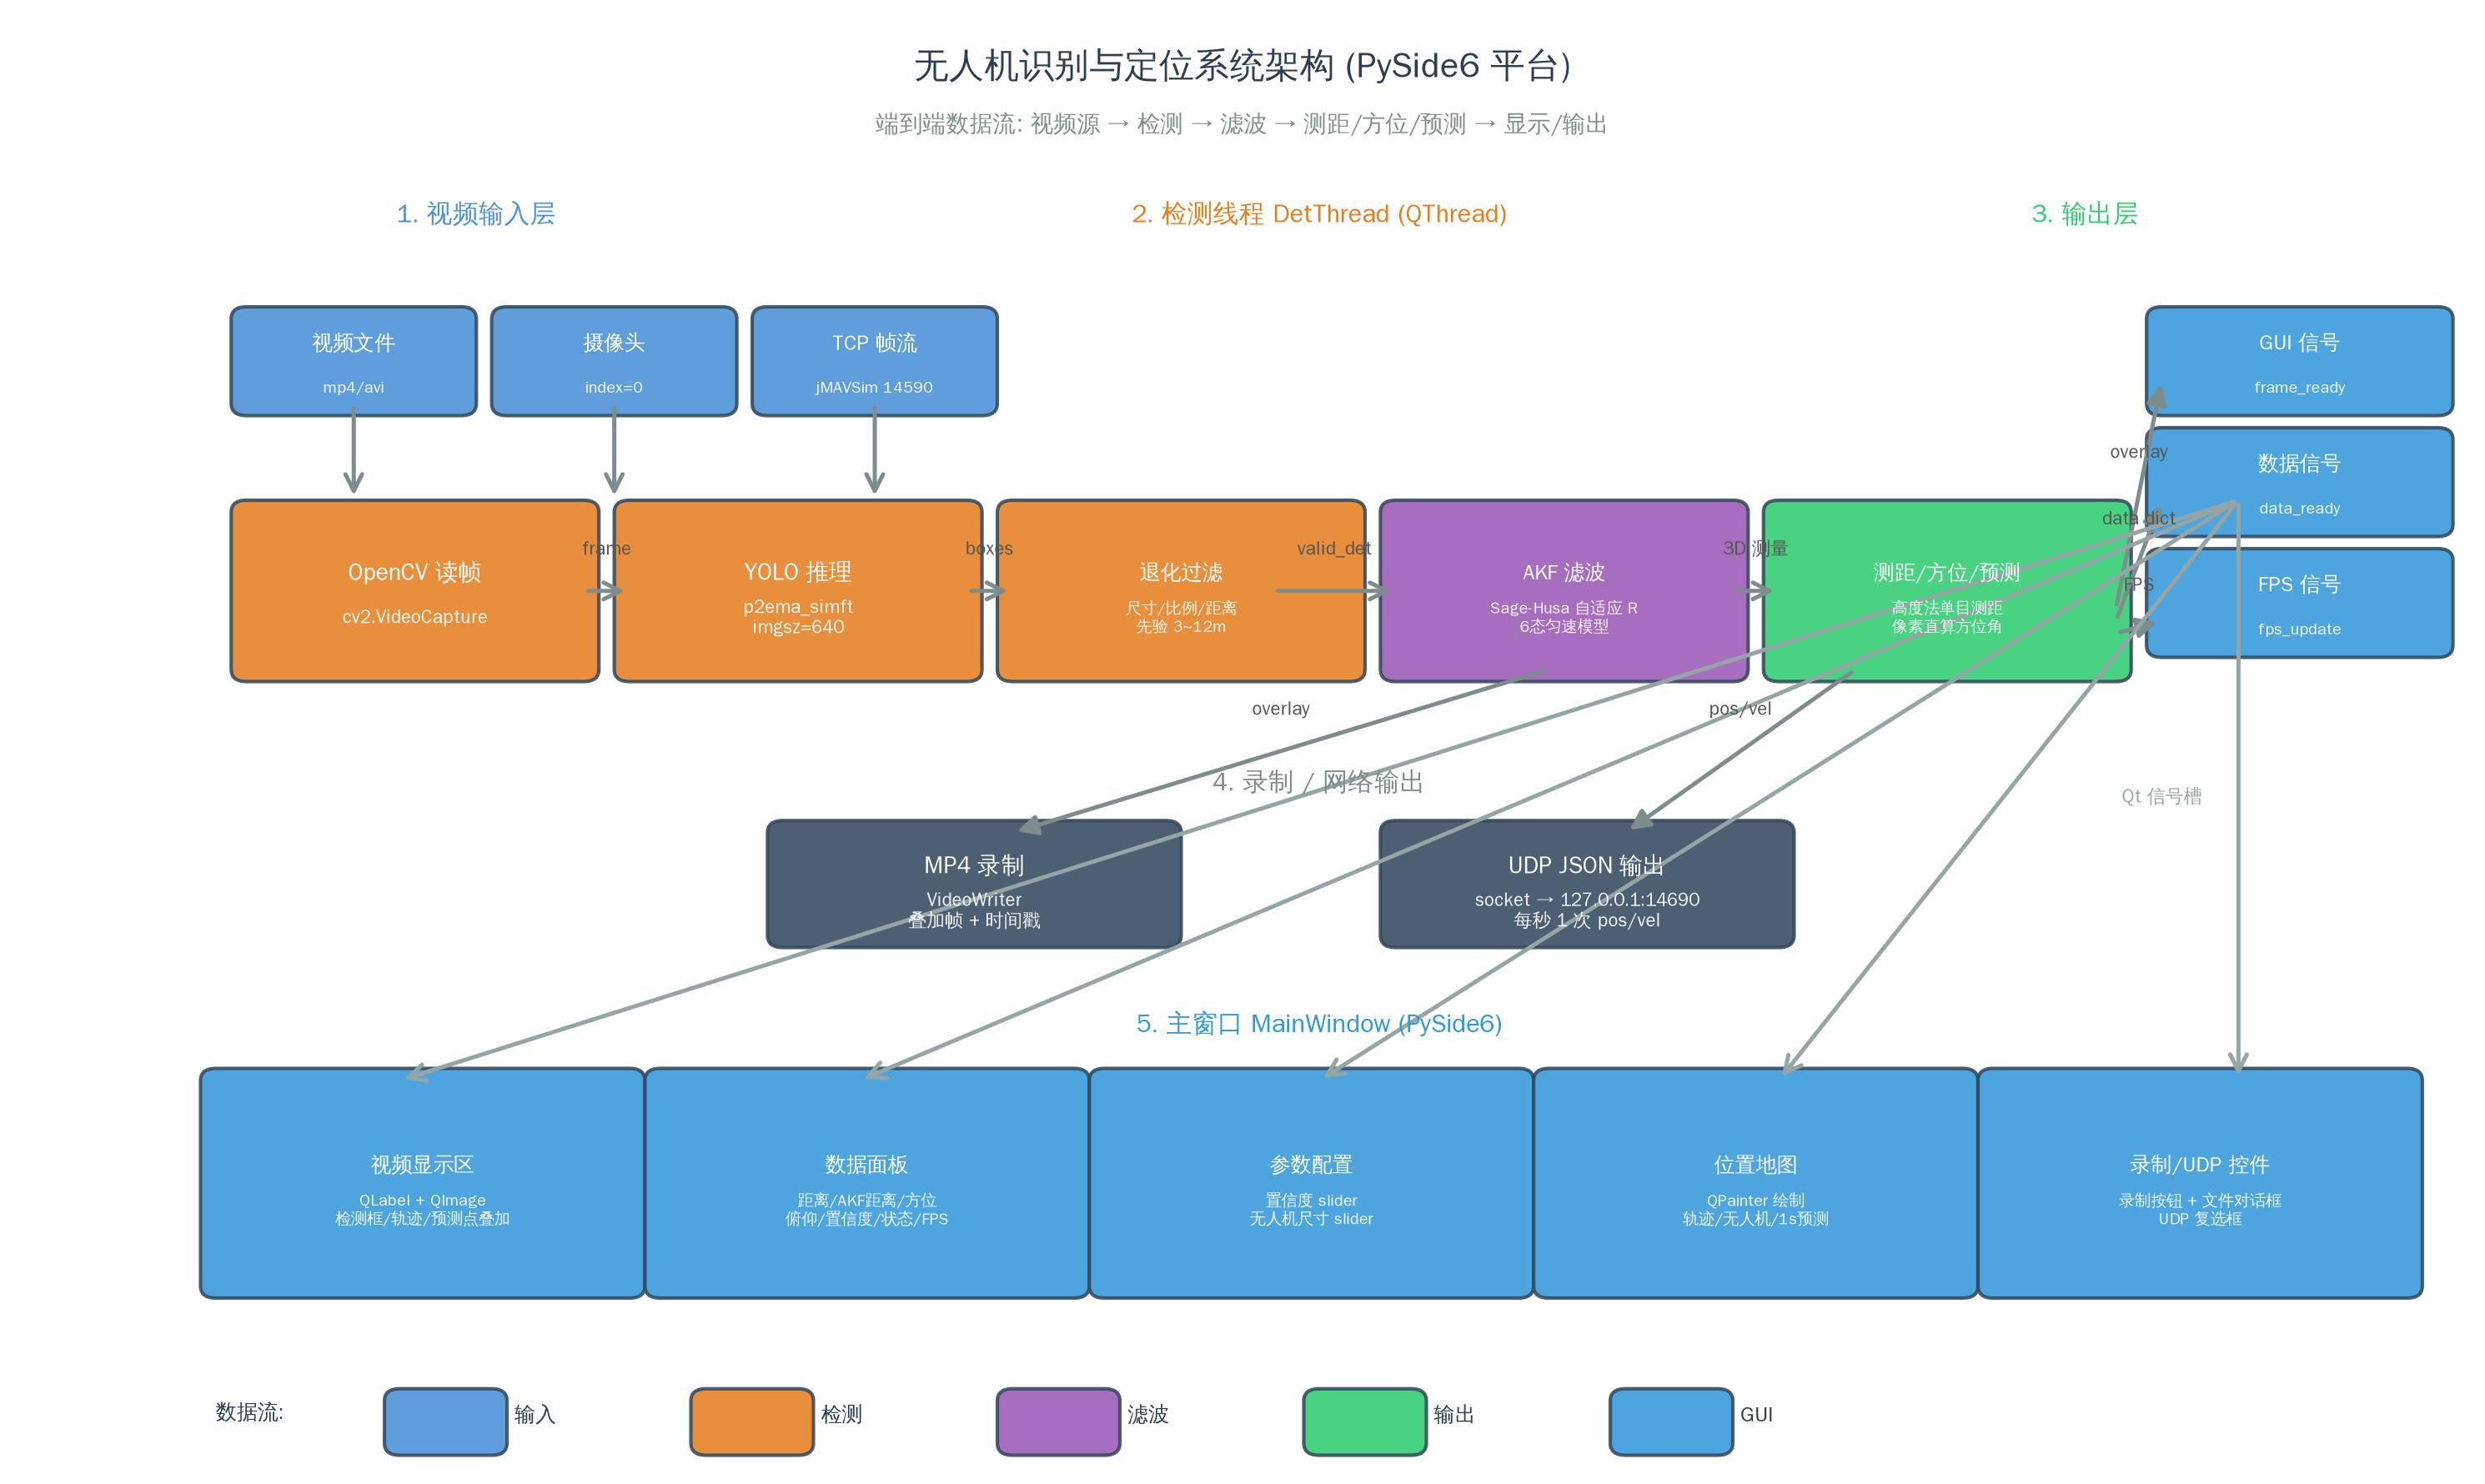
\includegraphics[width=0.9\textwidth]{system_arch.jpg}
  \caption{DRLS 系统架构与处理流水线}
  \label{fig:system_arch}
\end{figure}

\begin{enumerate}
  \item \textbf{检测环节}：采用 YOLOv8n + P2 + EMA 作为检测骨干
        （第~\ref{sec:model} 节），通过仿真域微调消除检测死区，
        使模型在 3--10\,m 全距离段具备可靠检出能力。

  \item \textbf{跟踪环节}：三态状态机对检测器原始输出进行滤波——
        初锁门限（0.55）防止误锁背景，维持门限（0.25）保证锁定稳定，
        空间门限（JUMP\_GATE = 140\,px）防止目标跳转，
        COAST 预算（1.0\,s）处理短时遮挡
        （第~\ref{sec:state_machine} 节）。

  \item \textbf{测距环节}：单目视觉测距公式
        $Z = f \cdot D_{\text{real}} / D_{\text{pixel}}$，
        AKF（Sage-Husa 自适应 R）对距离量测进行时域平滑，
        COAST 期间仅做预测步实现外推。

  \item \textbf{定位环节}：以锚点经纬度为原点，本机航向角为参考方向，
        目标方位角和距离为极坐标，通过 Haversine 公式
        转换为目标地理坐标，在卫星图上标注。

  \item \textbf{可视化环节}：PySide6 构建三页签桌面大屏，
        QWebEngineView 内嵌 Leaflet + Esri 卫星瓦片实现地图渲染，
        自绘 QWidget 实现罗盘仪表和数据条。
        所有控件数据通过 Qt 信号槽机制与后台检测线程实时联动。
\end{enumerate}

\subsection{系统界面}

DRLS 系统采用三页签大屏架构，目标态势页界面如图~\ref{fig:dashboard} 所示。

\begin{itemize}
  \item \textbf{目标态势页}（图~\ref{fig:dashboard_sat}）：左侧目标卡片显示
        目标类型、威胁等级、置信度与距离；中间区域为卫星图/雷达可切换的
        态势地图，实时标注目标位置与航迹；右侧为方位罗盘与距离仪表，
        配合底部 8 项数据条（AKF 距离、RAW 距离、方位角、俯仰角、置信度、
        状态、帧率、检出率）构成完整的态势感知界面。
        右下角 PIP（画中画）窗口实时显示带检测框的视频画面。

  \item \textbf{检测回放页}（图~\ref{fig:replay}）：支持录像文件回放与
        CSV 距离曲线联动，用于离线分析检测过程。

  \item \textbf{参数设置页}（图~\ref{fig:settings}）：提供置信度门限、
        无人机等效尺寸、TCP/UDP 地址、锚点坐标、本机航向、地图模式等
        参数的实时配置，所有设置自动持久化至 JSON 文件。
\end{itemize}

\begin{figure}[H]
  \centering
  \begin{subfigure}{0.48\textwidth}
    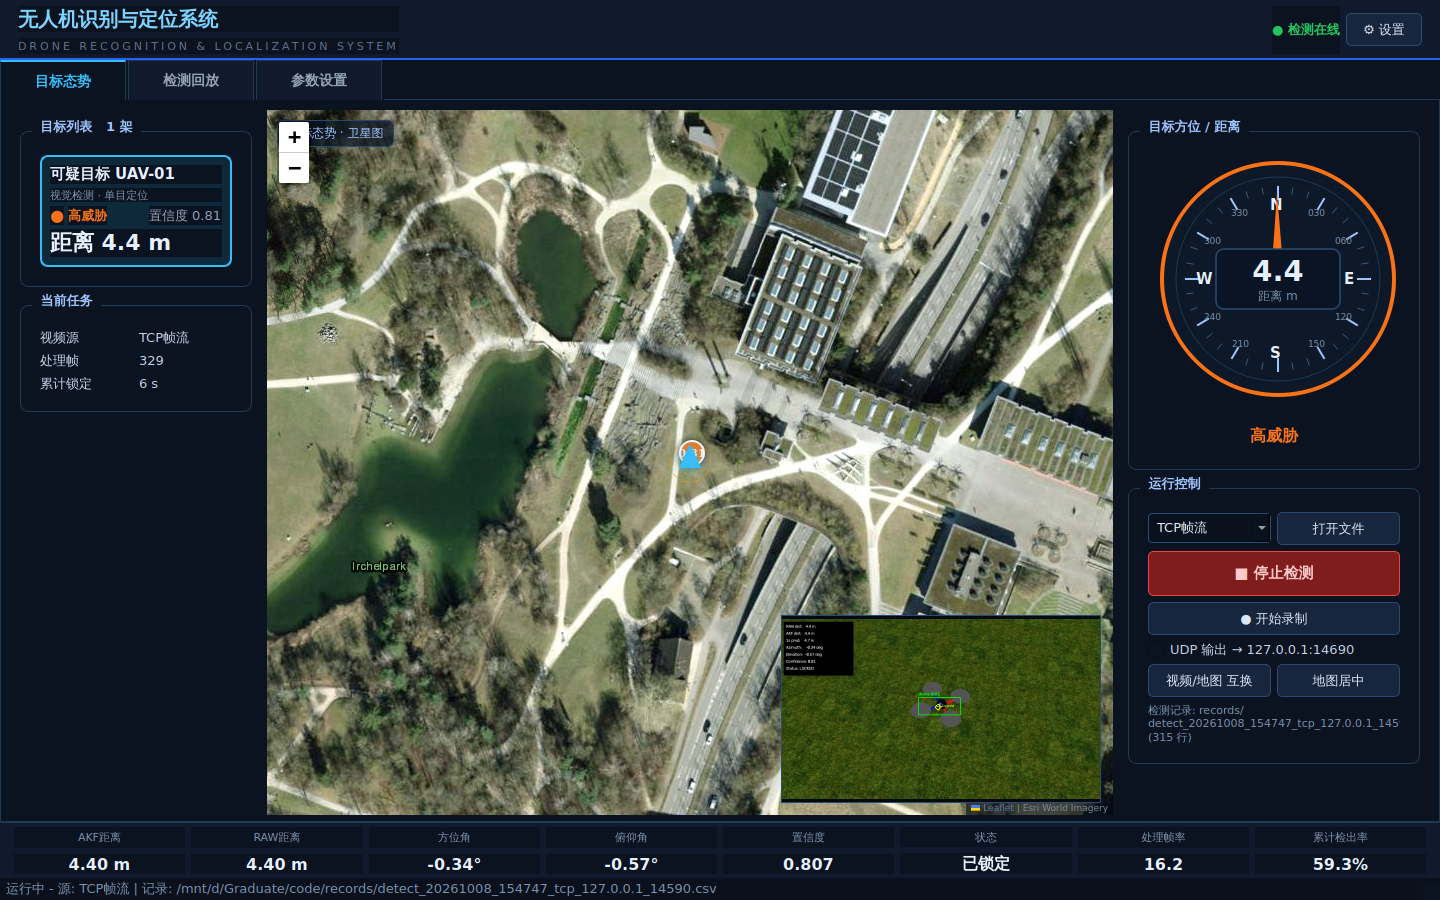
\includegraphics[width=\textwidth]{G_shot1_dashboard_satellite.png}
    \caption{卫星图模式（TCP 实时检测中）}
    \label{fig:dashboard_sat}
  \end{subfigure}
  \hfill
  \begin{subfigure}{0.48\textwidth}
    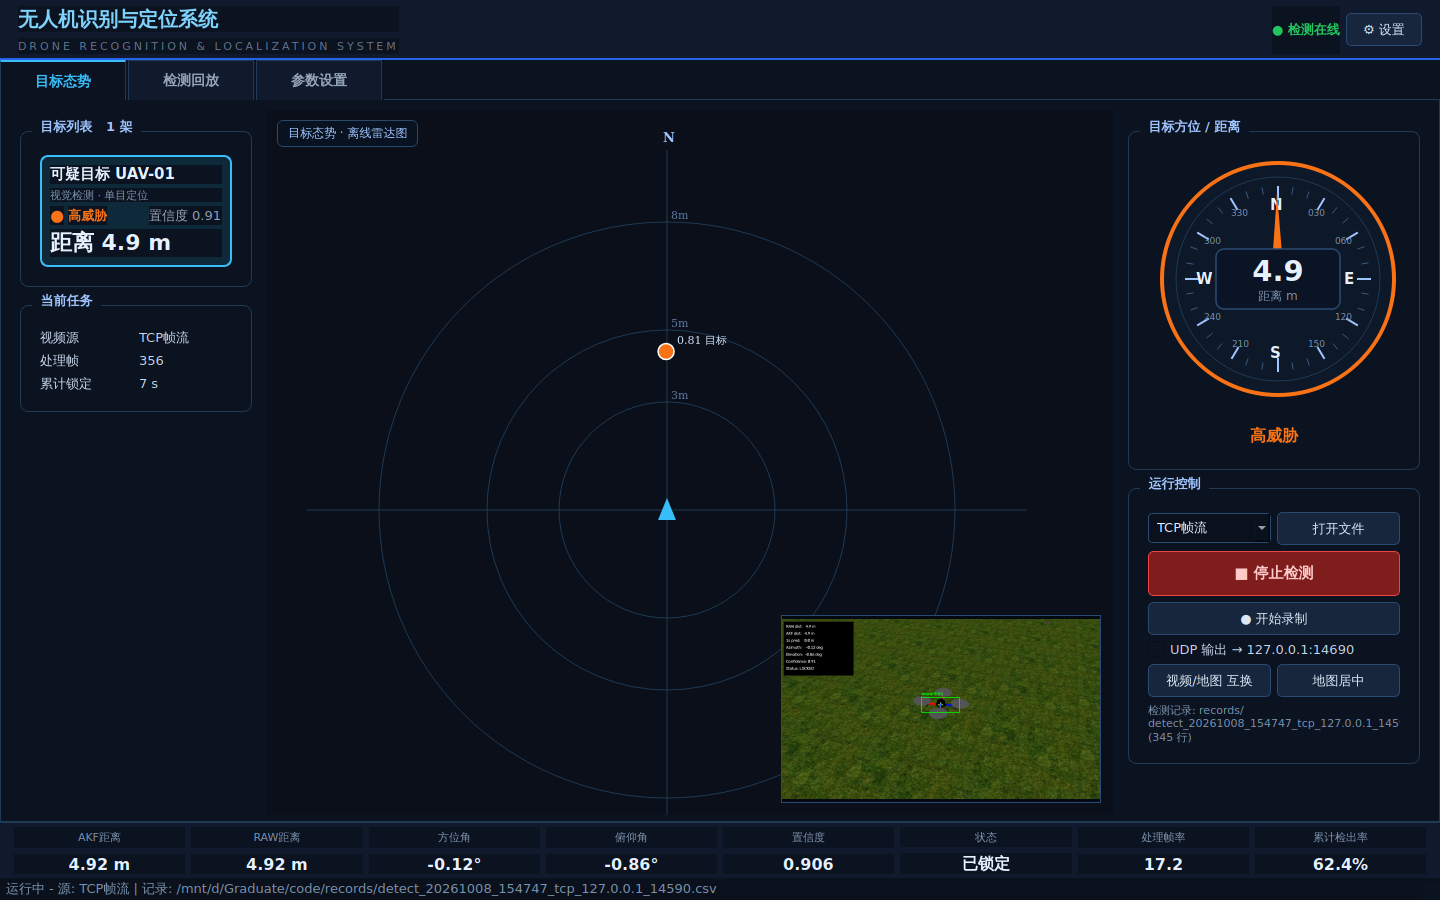
\includegraphics[width=\textwidth]{G_shot2_dashboard_radar.png}
    \caption{雷达模式（极坐标距离环）}
    \label{fig:dashboard_radar}
  \end{subfigure}
  \caption{目标态势页界面：左栏目标卡片、中地图/雷达、右罗盘仪表、底数据条}
  \label{fig:dashboard}
\end{figure}

\begin{figure}[H]
  \centering
  \begin{subfigure}{0.48\textwidth}
    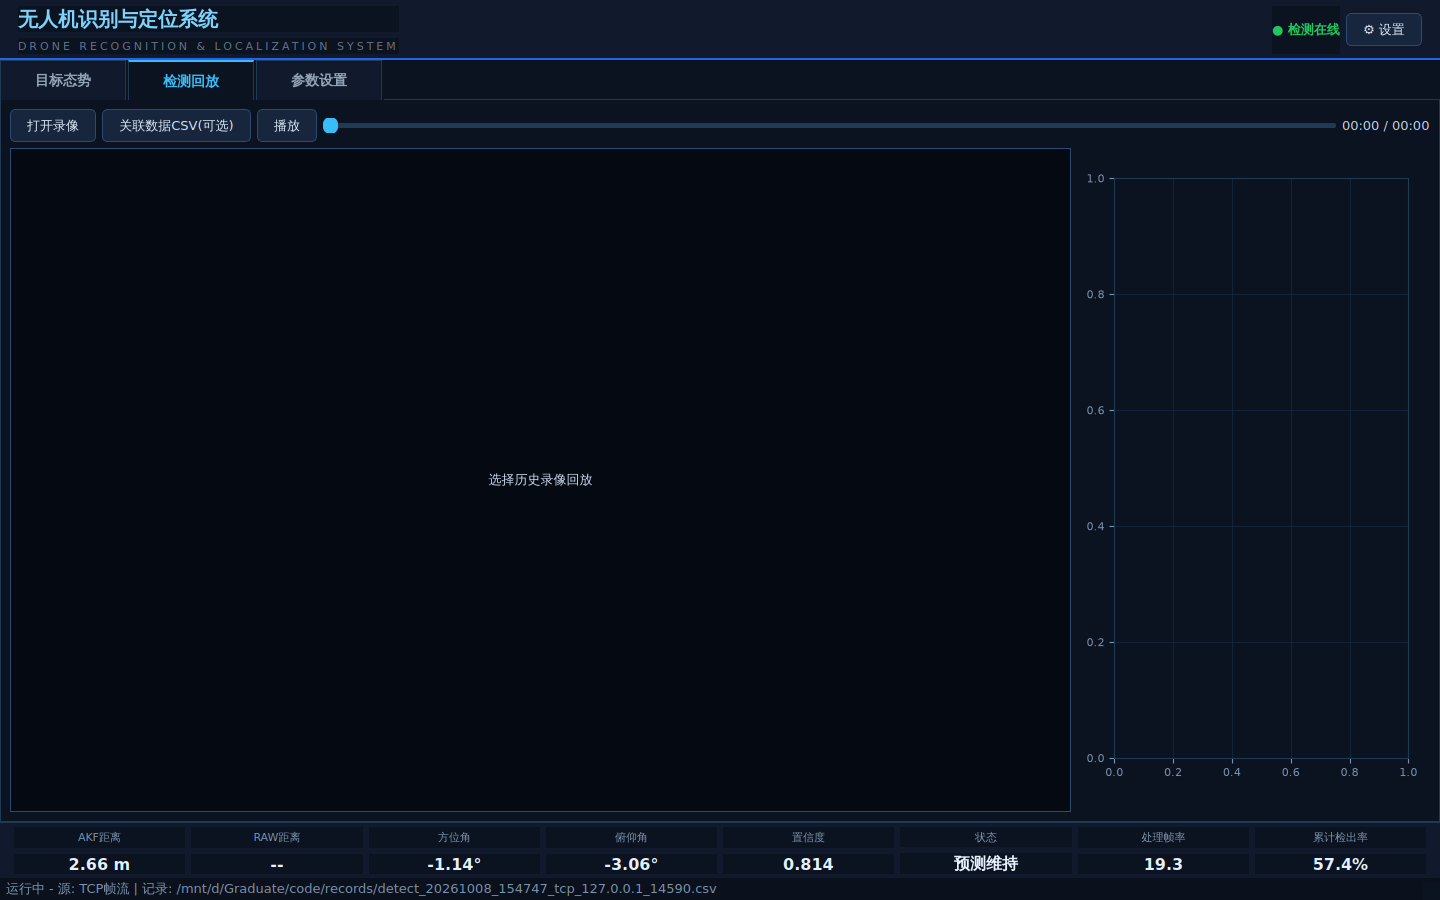
\includegraphics[width=\textwidth]{G_shot3_replay.png}
    \caption{检测回放页}
    \label{fig:replay}
  \end{subfigure}
  \hfill
  \begin{subfigure}{0.48\textwidth}
    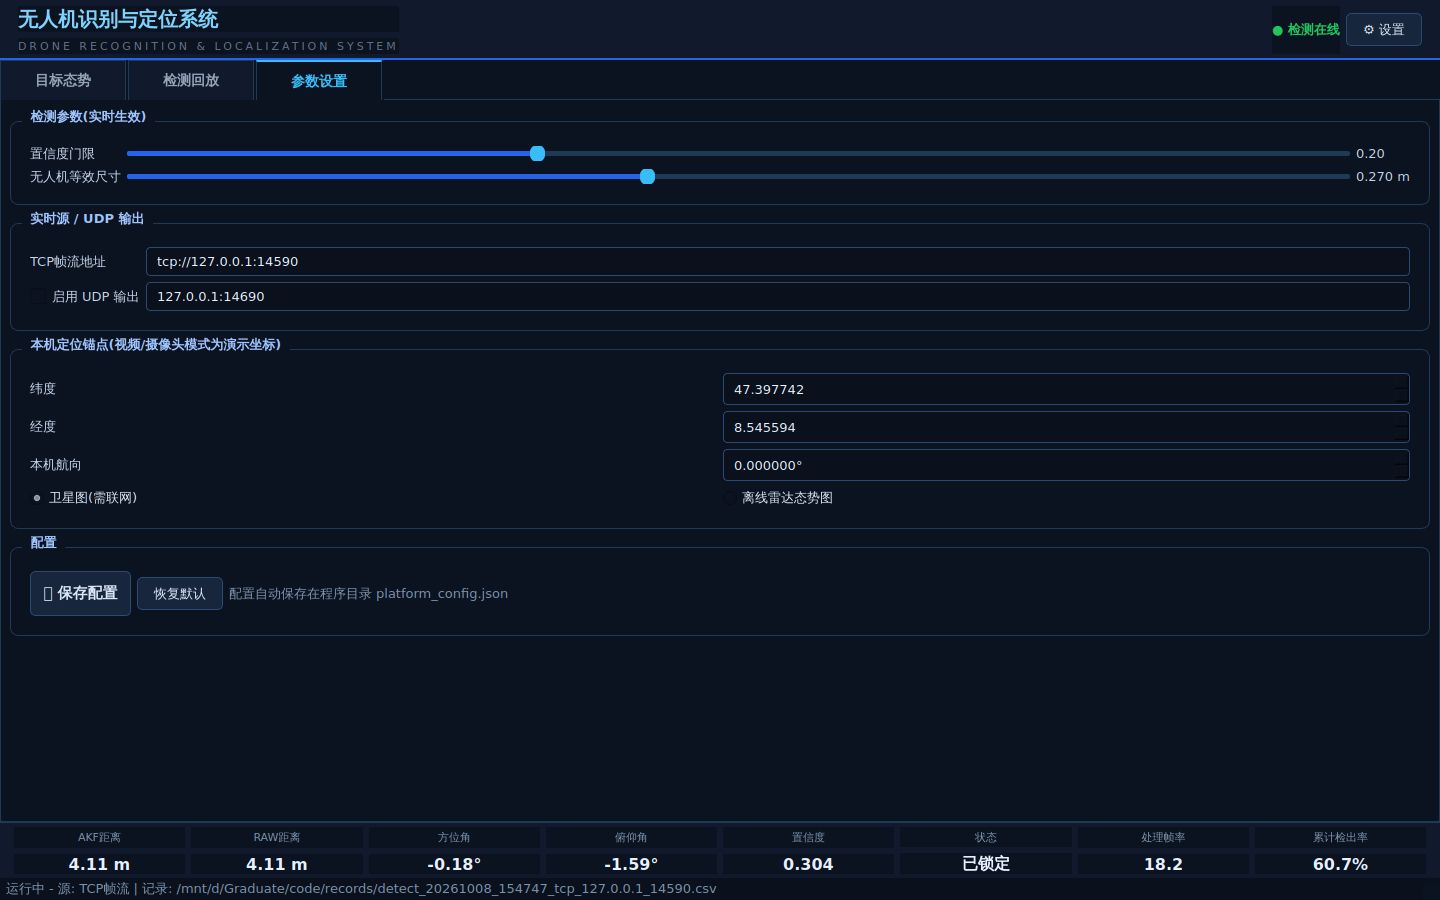
\includegraphics[width=\textwidth]{G_shot4_settings.png}
    \caption{参数设置页}
    \label{fig:settings}
  \end{subfigure}
  \caption{检测回放页与参数设置页界面}
  \label{fig:tabs23}
\end{figure}

%% ====================================================================
\section{检测模型与训练}
\label{sec:model}
%% ====================================================================

\subsection{模型选型与改进}

本文采用 YOLOv8n 作为目标检测骨干网络。YOLOv8 是 Ultralytics 公司
于 2023 年发布的单阶段目标检测算法，在 COCO 数据集上达到了当时的最优
精度-速度平衡。选择 YOLOv8n（nano 版本）的主要原因包括：
（1）实时性：在中端 GPU 上可达到 30\,fps 以上的推理速度；
（2）部署便捷：Ultralytics 框架提供简洁的 Python API，
便于嵌入 PySide6 桌面应用。

在反无人机场景中，目标无人机通常在远距离下成像尺寸极小
（检测框常 $< 50$\,px），属于典型的小目标检测问题。为提升对小目标的
检出率，本文在 YOLOv8n 基础上引入两项已被现有文献验证有效的改进：

\begin{enumerate}
  \item \textbf{P2 小目标检测头}：在原有三个检测层（P3/P4/P5）之外
        增加一个高分辨率 P2 检测层（stride=4），保留更多浅层空间细节。
        P2 检测层已在 SOD-YOLOv8\cite{sod_yolov8}、MSDF-Net\cite{msdf_net}
        等工作中被用于提升小目标检测精度。

  \item \textbf{EMA 注意力机制}：在 C2f 模块中嵌入高效多尺度注意力
        （Efficient Multi-scale Attention）\cite{ema}，通过分组并行子网络
        与跨空间聚合重新加权特征通道，增强目标响应、抑制背景干扰。
        EMA 已在 YOLOv8-MPEB\cite{yolov8_mpeb} 等工作中被验证有效。
\end{enumerate}

\textbf{需要说明的是}，P2 检测头与 EMA 注意力机制均为已有技术，
并非本文的创新点。本文的核心贡献在于构建一套面向反无人机场景的
完整识别与定位系统，包括：
\begin{itemize}
  \item 仿真域微调消除检测死区（第~\ref{subsubsec:deadzone} 节）；
  \item 三态跟踪状态机实现遮挡鲁棒性（第~\ref{sec:state_machine} 节）；
  \item 单目视觉测距与方位角估计（第~\ref{sec:state_machine} 节）；
  \item 态势可视化大屏与批量测试框架（第~\ref{sec:results} 节）。
\end{itemize}
P2+EMA 仅作为检测骨干的选型配置，为上述系统提供基础的检测能力。

\subsection{消融实验}

为验证 P2 检测头与 EMA 注意力机制对无人机小目标检测的增益效果，
本文在 Det-Fly 无人机检测数据集的验证集上进行了消融实验，
结果如表~\ref{tab:ablation} 所示。

\begin{table}[H]
\centering
\caption{检测骨干消融实验（Det-Fly 验证集，imgsz=640）}
\label{tab:ablation}
\small
\begin{tabular}{lccccccc}
\toprule
\textbf{模型} & \textbf{参数(M)} & \textbf{mAP50} & \textbf{mAP50-95} & \textbf{P(\%)} & \textbf{R(\%)} & \textbf{FPS} & \textbf{AP\_small} \\
\midrule
YOLOv8n（基线） & 3.01 & 81.3 & 41.8 & 91.2 & 75.9 & 123.0 & 6.1 \\
\quad+P2 & 2.93 & 82.3 & 41.3 & 88.9 & 77.6 & 90.3 & 8.3 \\
\quad+EMA & 3.02 & 76.2 & 36.3 & 85.5 & 72.2 & 101.0 & 4.1 \\
\quad\textbf{+P2+EMA} & 2.94 & \textbf{83.5} & 41.2 & 88.2 & \textbf{79.2} & 98.4 & \textbf{9.8} \\
\bottomrule
\end{tabular}
\end{table}

分析：

\begin{enumerate}
  \item \textbf{P2 检测头}：单独加入 P2 后，mAP50 从 81.3\% 提升至 82.3\%，
        小目标 AP（AP\_small）从 6.1\% 提升至 8.3\%（+2.2\,pp），
        召回率从 75.9\% 提升至 77.6\%。
        这表明 P2 高分辨率检测层确实有助于捕获小目标特征。
        但 mAP50-95 略降（41.8\%$\rightarrow$41.3\%），
        说明 P2 引入的浅层特征可能对大中目标的精确定位有轻微干扰。

  \item \textbf{EMA 注意力}：单独加入 EMA 后，mAP50 从 81.3\% 下降至 76.2\%，
        AP\_small 从 6.1\% 降至 4.1\%。
        这表明 EMA 在 Det-Fly 数据集上单独使用时反而引入了负面影响，
        可能是因为 EMA 的特征重分布在通用无人机数据集上过度抑制了
        部分有效响应。

  \item \textbf{P2+EMA 联合}：二者联合使用后，mAP50 达到最优的 83.5\%
        （+2.2\,pp），AP\_small 达到 9.8\%（+3.7\,pp），
        召回率达到 79.2\%（+3.3\,pp）。
        这表明 P2 的高分辨率特征与 EMA 的注意力重分布存在协同效应：
        P2 提供了更丰富的浅层空间信息，使 EMA 有更多有效特征可加权，
        从而克服了 EMA 单独使用时的信息损失问题。
\end{enumerate}

综合以上结果，本文选择 P2+EMA 配置作为检测骨干。参数量 2.94\,M
（略低于基线的 3.01\,M），推理速度 98.4\,fps 满足实时性要求。

\subsection{数据集与训练策略}

模型训练分为两个阶段：

\begin{enumerate}
  \item \textbf{预训练阶段}：在通用无人机检测数据集上进行预训练，
        学习无人机的基本外观特征（旋翼、机身、机臂比例等）。

  \item \textbf{仿真微调阶段}：采集 jMAVSim 仿真场景下的无人机图像，
        标注后进行领域自适应微调（Domain Adaptation Fine-tuning），
        使模型更好地适应仿真环境的视觉特征（光照、背景纹理、目标尺寸分布）。
        微调后的模型记为 \texttt{p2ema\_simft}。
\end{enumerate}

\subsubsection{微调前后检测死区对比}
\label{subsubsec:deadzone}

为验证仿真域微调的必要性，本文在闭环仿真环境中对比了微调前后的检出率。
使用同一仿真轨迹录像（距离范围 3.2--9.1\,m），分别用微调前模型
（\texttt{p2ema}，仅在 Det-Fly 数据集上训练）和微调后模型
（\texttt{p2ema\_simft}）进行逐帧检测，按距离段统计检出率，
结果如表~\ref{tab:finetune_compare} 所示。

\begin{table}[H]
\centering
\caption{仿真域微调前后检出率对比（按距离段）}
\label{tab:finetune_compare}
\small
\begin{tabular}{p{1.5cm}p{1.2cm}p{1.0cm}p{1.2cm}p{1.2cm}p{1.0cm}p{1.2cm}}
\toprule
\multirow{2}{*}{\textbf{距离段}} & \multicolumn{3}{c}{\textbf{微调前（p2ema）}} & \multicolumn{3}{c}{\textbf{微调后（p2ema\_simft）}} \\
\cmidrule(lr){2-4} \cmidrule(lr){5-7}
 & 帧数 & 检出 & 检出率 & 帧数 & 检出 & 检出率 \\
\midrule
3--4\,m & 289 & 0 & \textbf{0.0\%} & 367 & 367 & 100.0\% \\
4--5\,m & 224 & 0 & \textbf{0.0\%} & 267 & 267 & 100.0\% \\
5--6\,m & 202 & 9 & 4.5\% & 224 & 224 & 100.0\% \\
6--7\,m & 797 & 59 & 7.4\% & 980 & 980 & 100.0\% \\
7--8\,m & 270 & 78 & 28.9\% & 366 & 366 & 100.0\% \\
8--9\,m & 356 & 77 & 21.6\% & 491 & 491 & 100.0\% \\
9--10\,m & 90 & 0 & \textbf{0.0\%} & 123 & 123 & 100.0\% \\
\midrule
\textbf{合计} & 2228 & 223 & \textbf{10.0\%} & 2818 & 2818 & \textbf{100.0\%} \\
\bottomrule
\end{tabular}
\end{table}

微调前模型存在明显的"检测死区"现象：

\begin{itemize}
  \item \textbf{近距死区（3--5\,m）}：检出率 0\%。目标无人机在此距离下
        成像尺寸较大，超出 Det-Fly 训练集的目标尺寸分布范围
        （分布外，Out-of-Distribution），模型无法识别。

  \item \textbf{远距死区（9--10\,m）}：检出率 0\%。目标成像尺寸过小
        （检测框 $< 50$\,px），模型可提取的特征不足。

  \item \textbf{有效工作窗口（7--9\,m）}：仅在此距离范围内模型具有一定的
        检出能力（21.6\%--28.9\%），但远未达到实用水平。
\end{itemize}

微调后，模型在全部距离段（3--10\,m）的检出率均提升至 100\%，
死区完全消除。这表明仿真域微调有效弥补了预训练模型在仿真视觉域的
分布外问题，使模型在 3--10\,m 的全距离范围内具备可靠的检测能力。

\textbf{需要说明的是}，上述 100\% 检出率是在固定轨迹、无遮挡物的
理想仿真条件下获得的。在本文第~\ref{sec:results} 节的 14 用例测试中，
引入随机航迹与遮挡物后，系统的锁定率（LOCKED 帧占比）下降至
55--59\%，但航迹保持率（含 COAST 预测）仍维持在 89--95\%，
更真实地反映了系统在复杂场景下的跟踪能力。
此外，仿真轨迹仅覆盖 3--10\,m 距离范围，
10\,m 以上的检测性能由真实场景录像 C05 标定
（详见第~\ref{subsec:real_scenario} 节）。

训练曲线如图~\ref{fig:training} 所示，模型在训练过程中损失函数稳定下降，
精度（Precision）和召回率（Recall）均收敛至较高水平。

\begin{figure}[H]
  \centering
  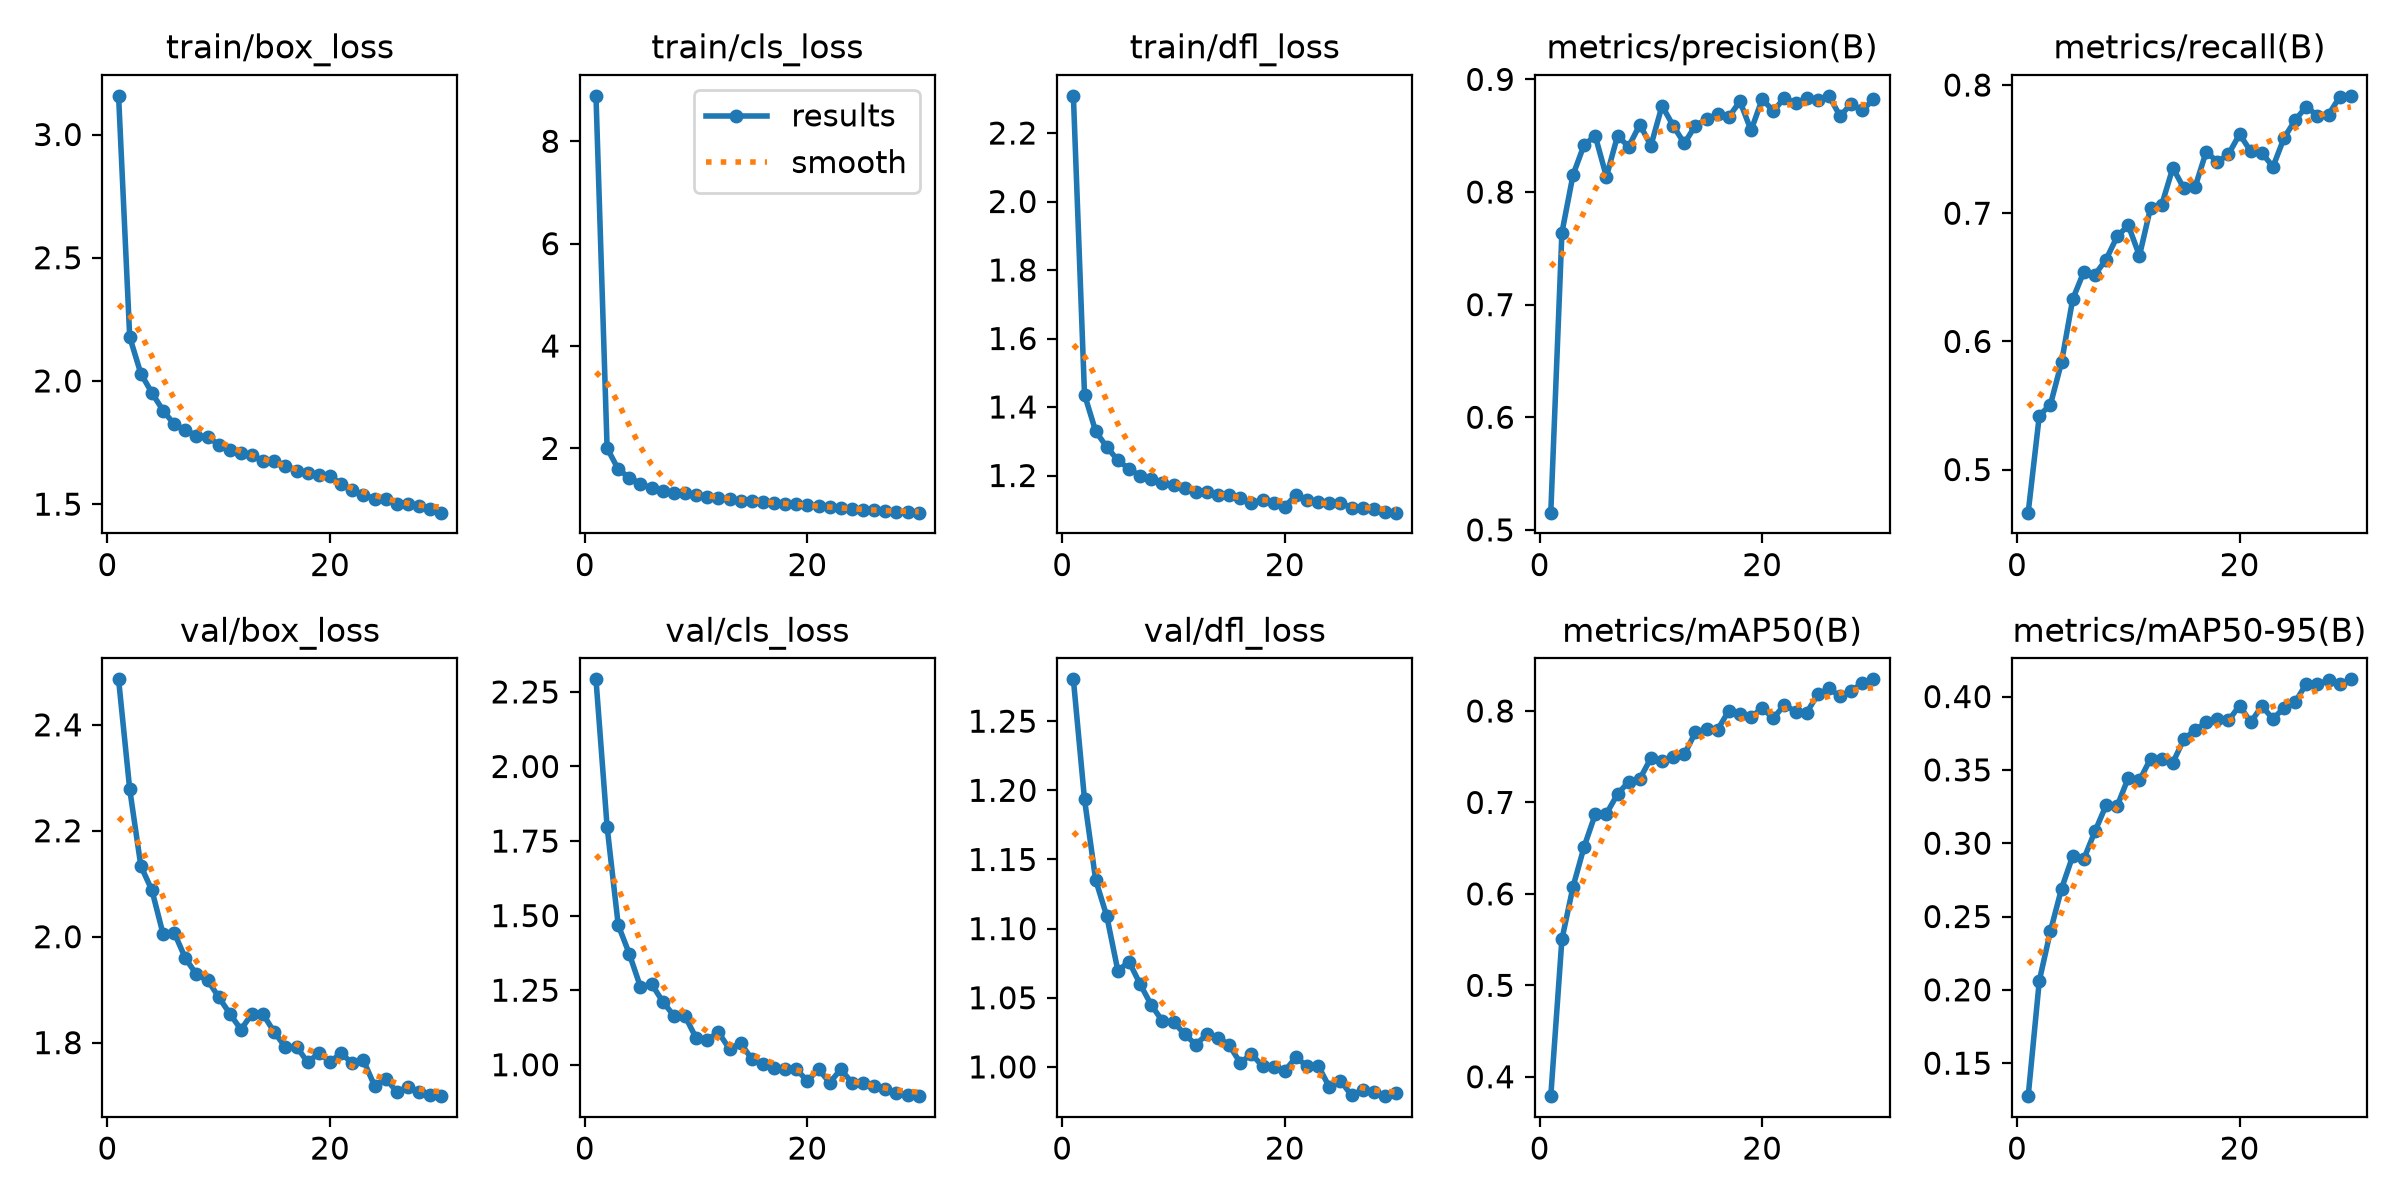
\includegraphics[width=0.85\textwidth]{training_curves_p2ema.png}
  \caption{模型训练曲线（损失、精度、召回率）}
  \label{fig:training}
\end{figure}

\subsection{模型评估}

在验证集上，微调后模型的 PR 曲线如图~\ref{fig:pr_curve} 所示，
混淆矩阵如图~\ref{fig:confusion} 所示。

\begin{figure}[H]
  \centering
  \begin{subfigure}{0.48\textwidth}
    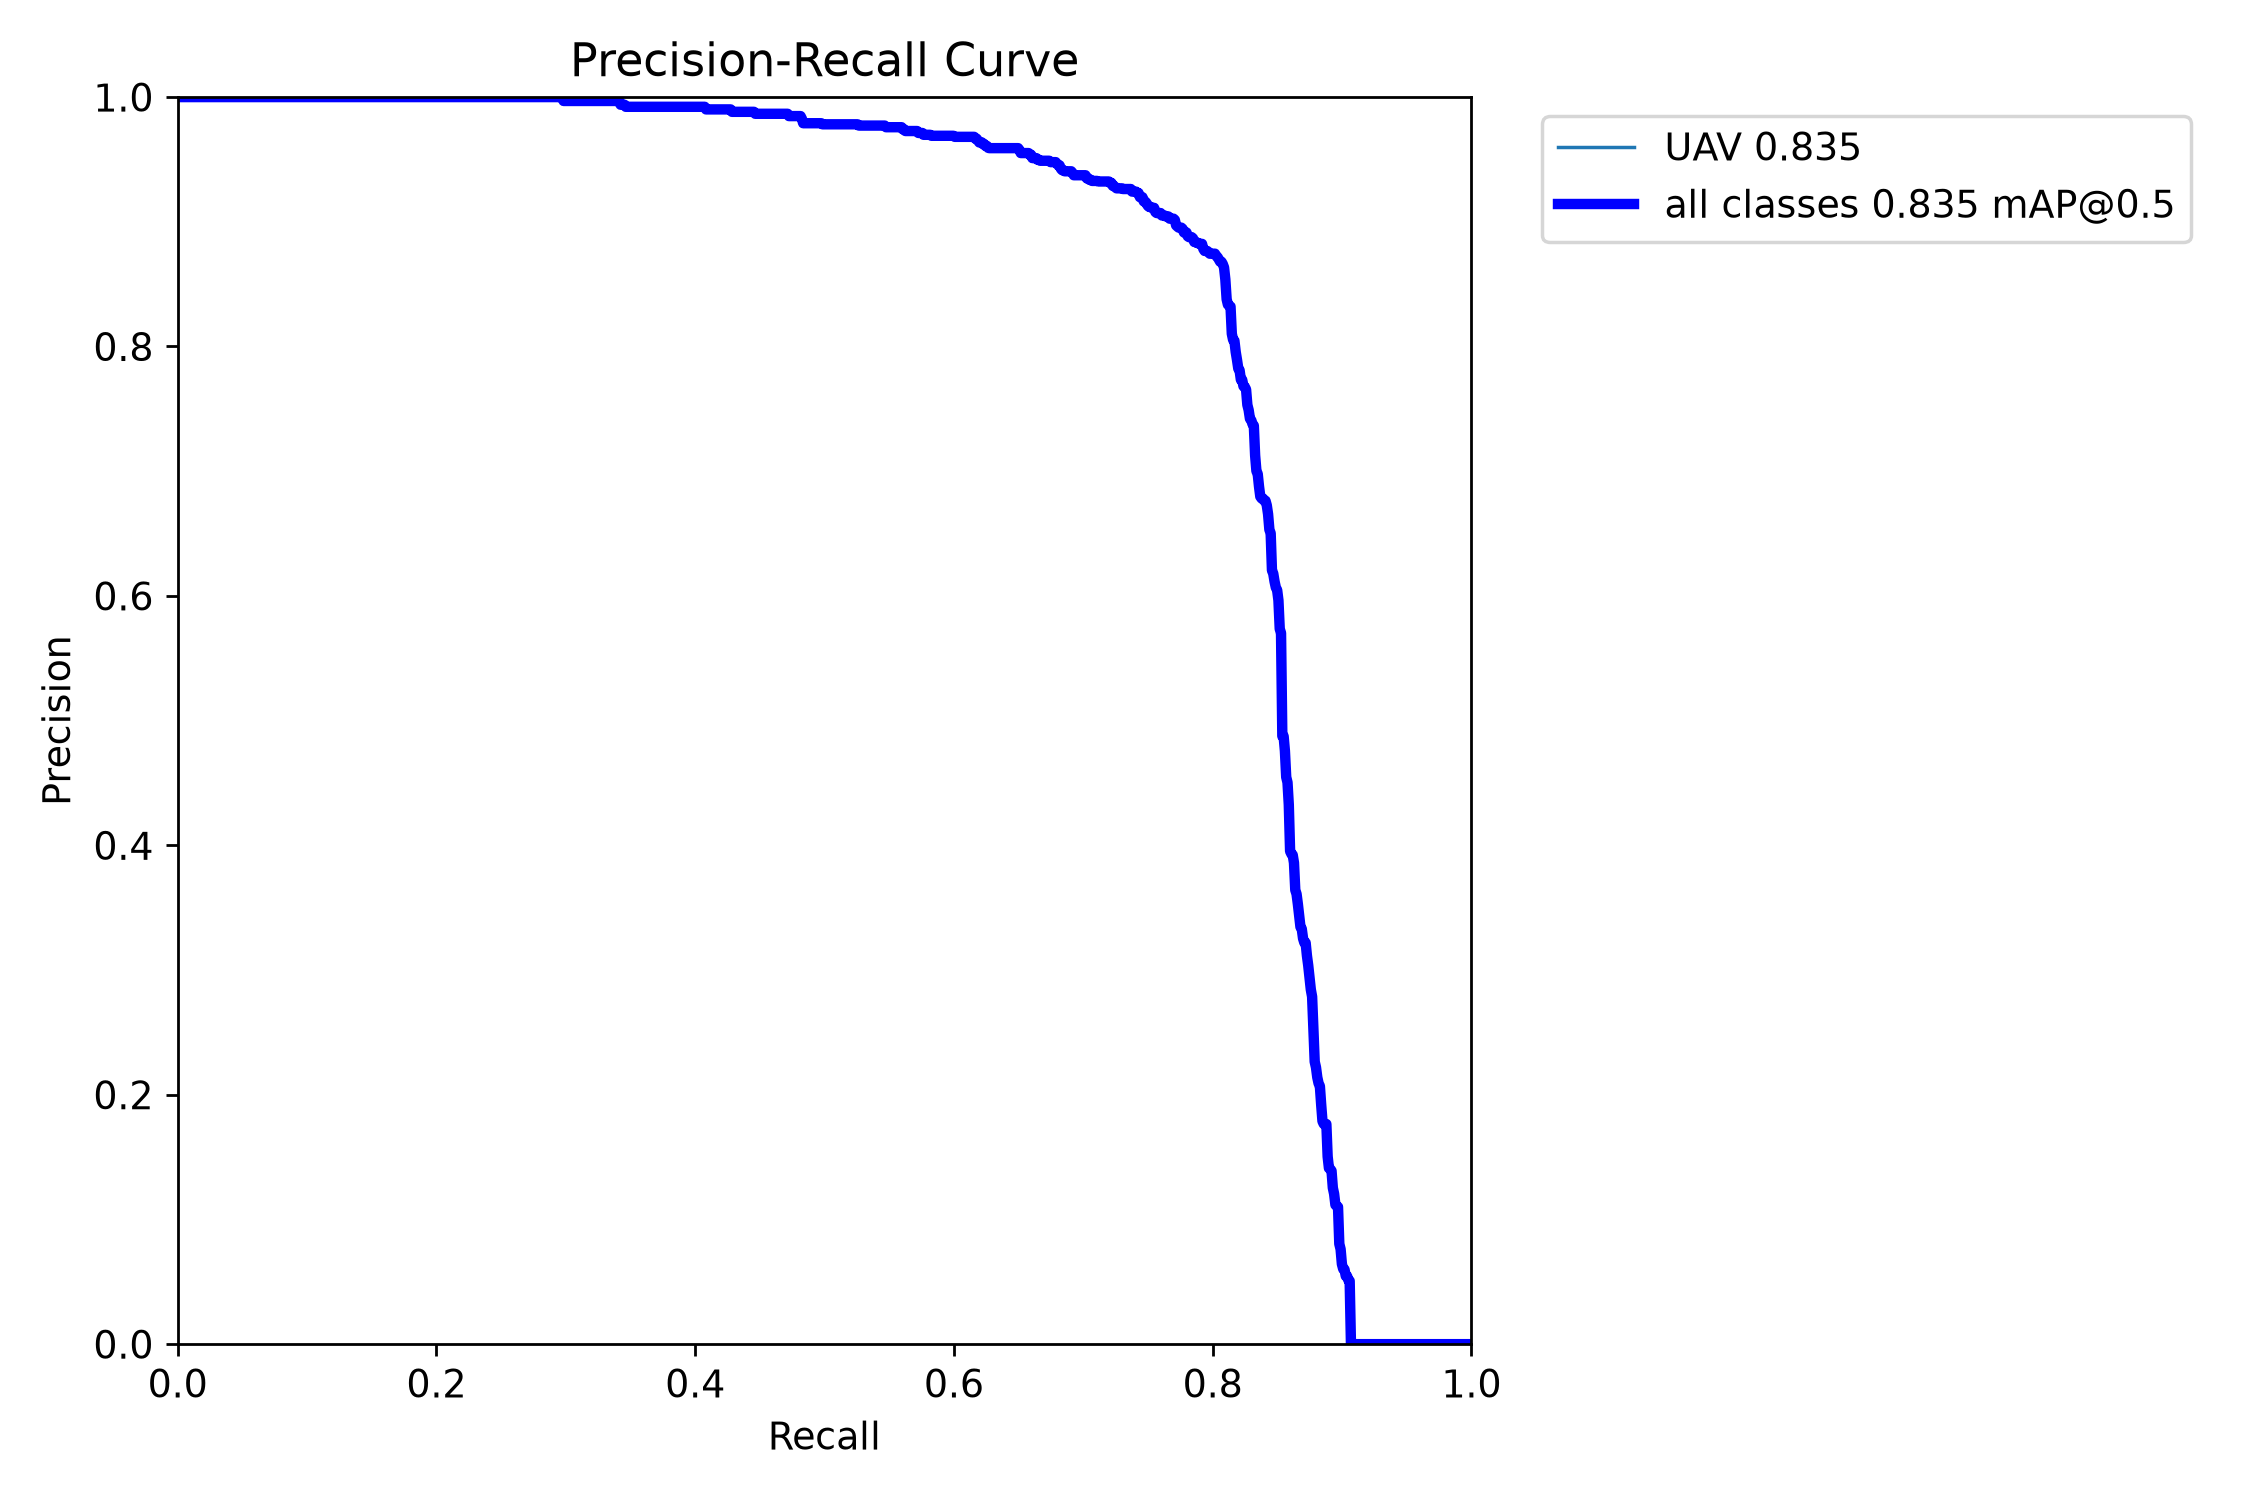
\includegraphics[width=\textwidth]{pr_curve_p2ema.png}
    \caption{PR 曲线}
    \label{fig:pr_curve}
  \end{subfigure}
  \hfill
  \begin{subfigure}{0.48\textwidth}
    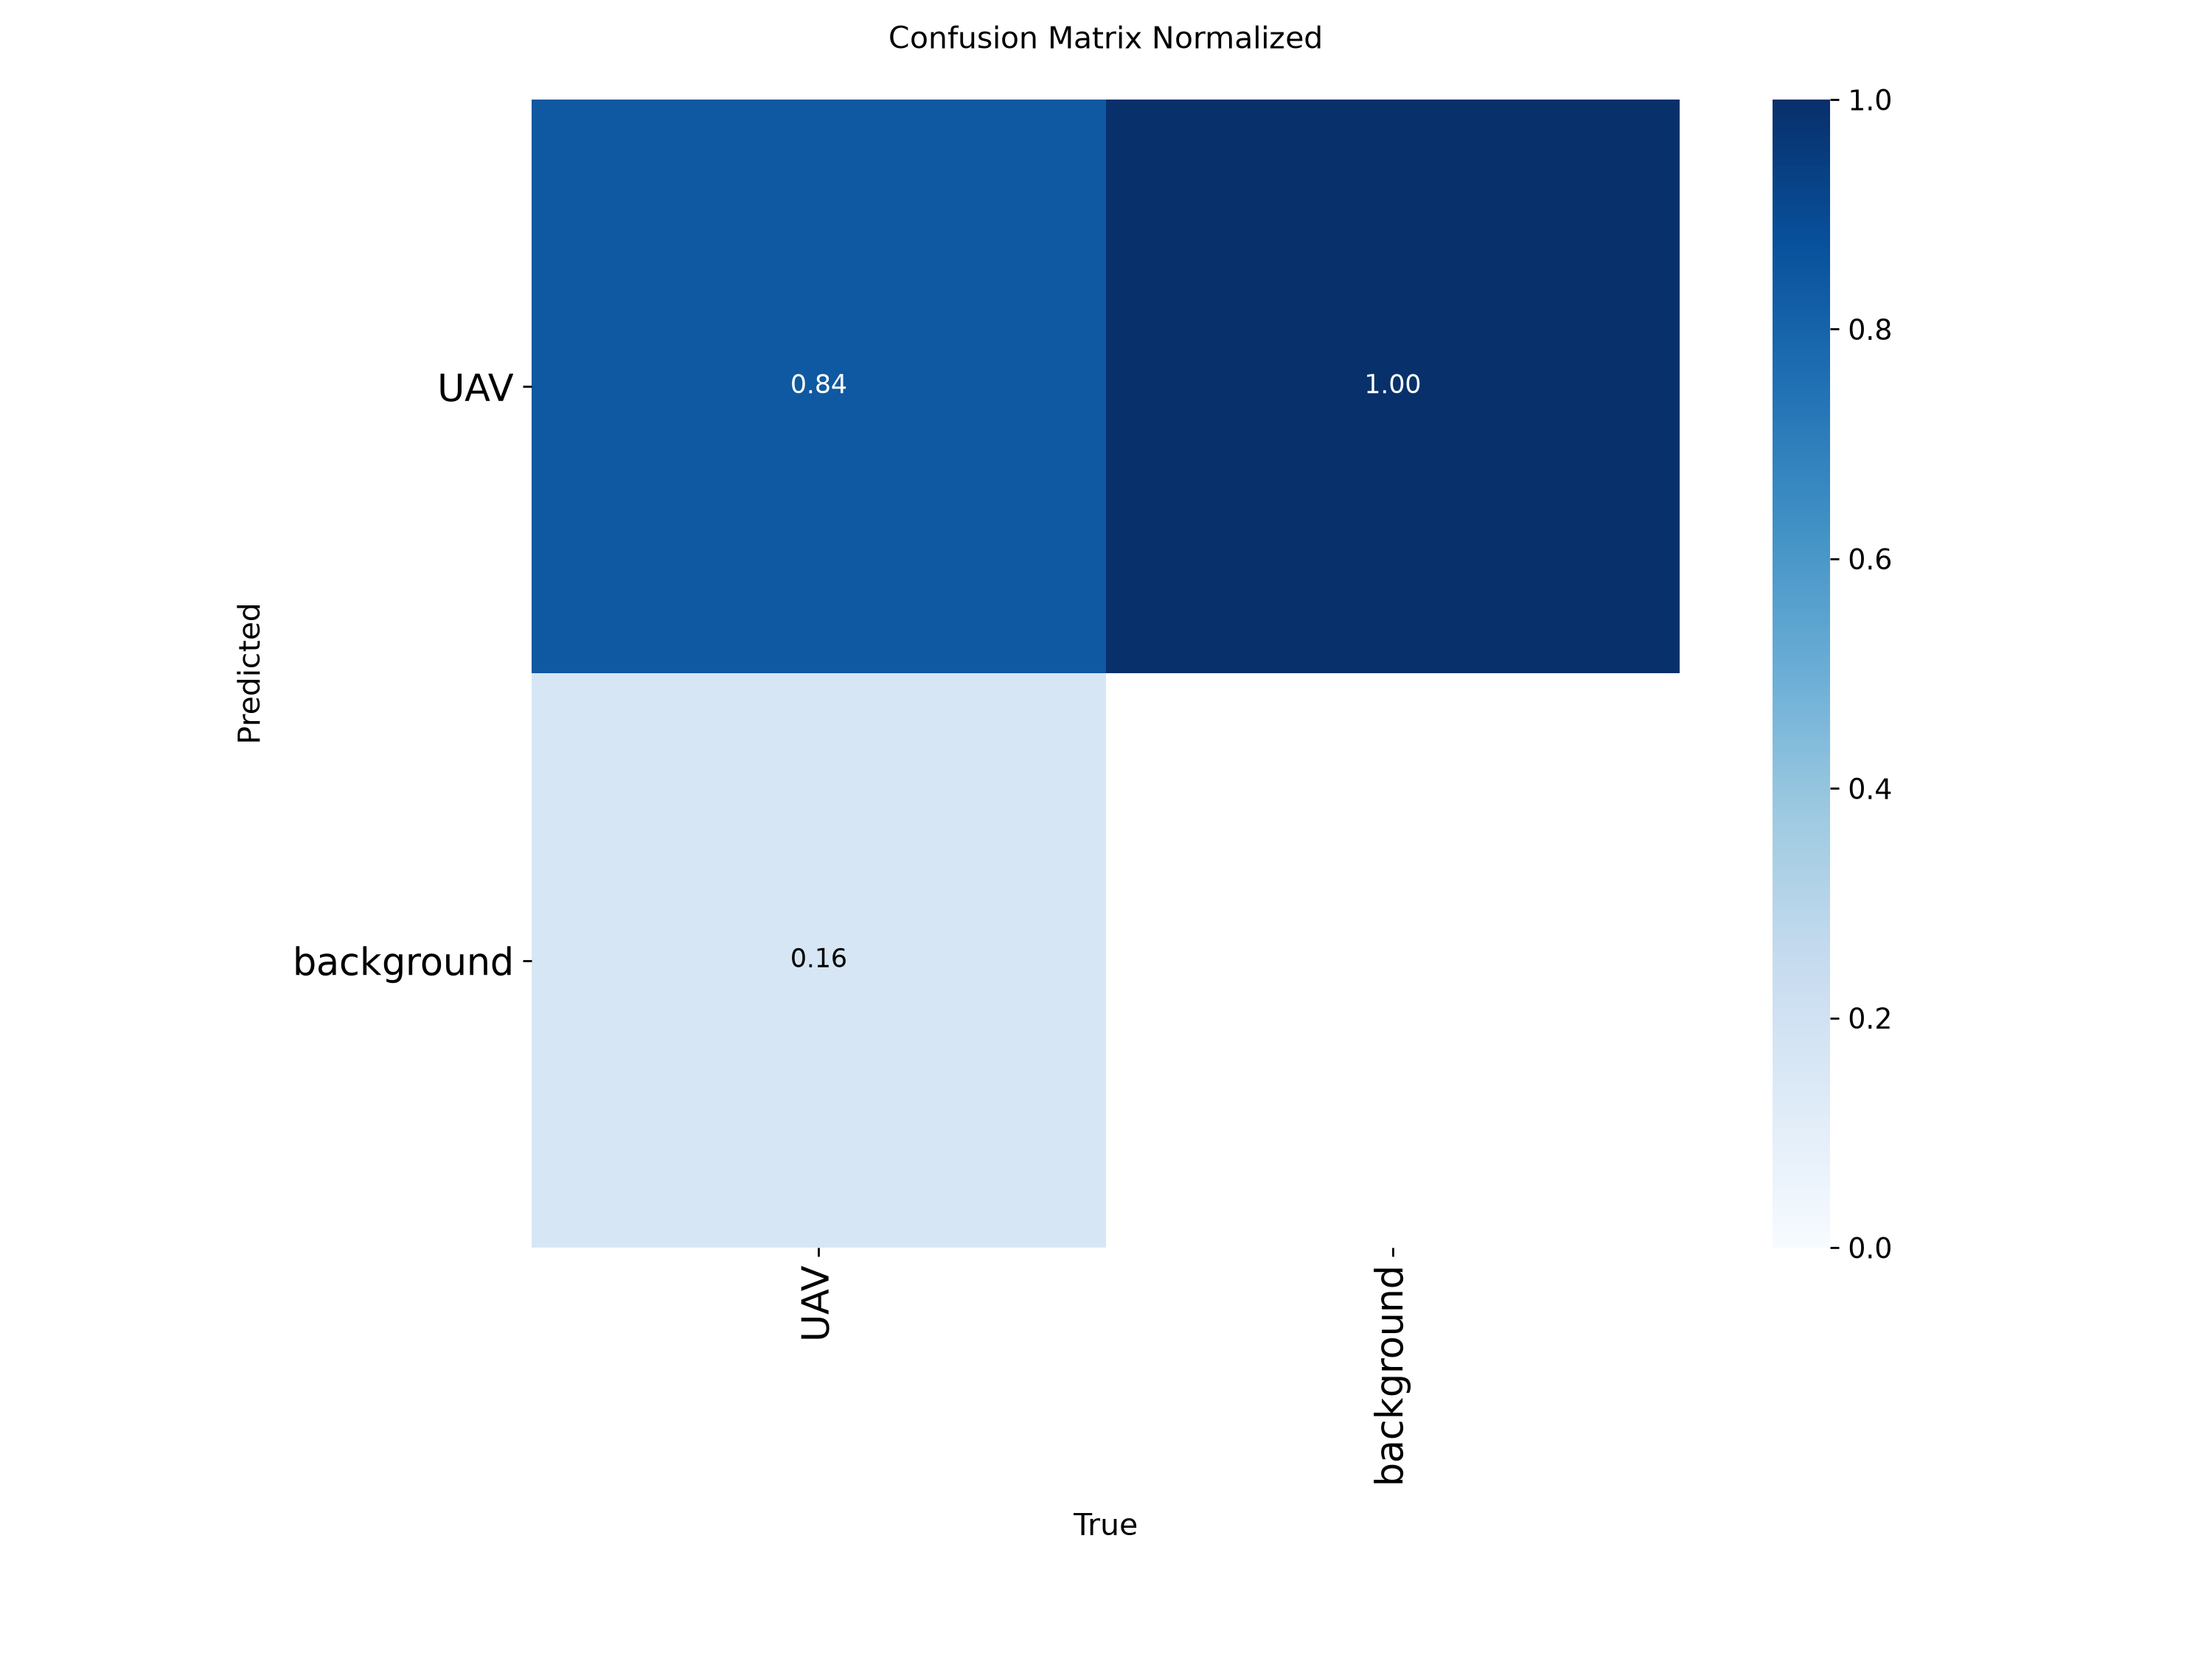
\includegraphics[width=\textwidth]{confusion_matrix_p2ema.png}
    \caption{混淆矩阵}
    \label{fig:confusion}
  \end{subfigure}
  \caption{模型在验证集上的评估结果}
  \label{fig:model_eval}
\end{figure}

%% ====================================================================
\section{目标跟踪状态机设计}
\label{sec:state_machine}
%% ====================================================================

\subsection{状态机设计动机}

在原始的逐帧检测方案中，系统每帧独立选取置信度最高的检测框作为目标，
存在以下问题：

\begin{enumerate}
  \item \textbf{误锁背景}：当画面中出现高置信度的非目标物体时，
        系统会误将其锁定为目标。
  \item \textbf{数据断闪}：目标短暂被遮挡时，检测器无法输出检测框，
        导致距离、方位等数据瞬间清零，用户体验差。
  \item \textbf{无法预测**}：丢失目标后系统无任何预测能力，
        无法为下游系统（如 UDP 输出）提供连续的态势数据。
\end{enumerate}

为解决上述问题，本文设计了一种三态跟踪状态机，将检测器的原始输出
经过状态机滤波后输出稳定的跟踪结果。

\subsection{三态状态机}

状态机包含三个状态：搜索中（SEARCH）、已锁定（LOCKED）和预测维持（COAST），
状态转移条件如表~\ref{tab:state_machine} 所示。

\begin{table}[H]
\centering
\caption{跟踪状态机状态转移条件}
\label{tab:state_machine}
\begin{tabular}{p{2cm}p{3.5cm}p{4cm}p{4cm}}
\toprule
\textbf{状态} & \textbf{进入条件} & \textbf{维持条件} & \textbf{退出条件} \\
\midrule
搜索中 (SEARCH) & 初始状态 & 无有效候选 & 候选置信度 $> 0.55$（初锁门限） \\
已锁定 (LOCKED) & 候选置信度 $> 0.55$ 且距上一帧目标中心 $< 140$\,px & 候选置信度 $> 0.25$（维持门限）且像素跳变 $< 140$\,px & 置信度 $< 0.25$ 或无检测框 \\
预测维持 (COAST) & LOCKED 状态下丢失目标 & 卡尔曼滤波器外推，预算 $T_{\text{coast}} = 1.0$\,s & 目标重新出现$\rightarrow$LOCKED；超时$\rightarrow$SEARCH \\
\bottomrule
\end{tabular}
\end{table}

状态机的核心设计要点包括：

\begin{enumerate}
  \item \textbf{双门限策略}：初锁门限（$0.55$）高于维持门限（$0.25$），
        前者防止误锁背景，后者保证目标被锁定后即使置信度波动也不会
        频繁丢失锁定。

  \item \textbf{空间门限（JUMP\_GATE）}：LOCKED 状态下只接受距上一帧
        目标中心 $140$\,像素以内的检测框，防止目标"跳"到画面中的
        其他物体上。测距突变超过 $1.4$ 倍的异常量测会被
        Z\_GATE 拒绝，连续拒绝触发滤波器重置。

  \item \textbf{COAST 预算}：丢失目标后用卡尔曼滤波器预测外推
        $T_{\text{coast}} = 1.0$\,s（初始值 $0.6$\,s，后经实验优化，
        详见第~\ref{subsec:coast_opt} 节）。超时后回到 SEARCH 状态。
\end{enumerate}

\subsection{卡尔曼滤波}

在 LOCKED 和 COAST 状态下，系统使用卡尔曼滤波器对距离量测进行平滑。
状态向量包括距离及其变化率：
\[
\mathbf{x} = \begin{bmatrix} z \\ \dot{z} \end{bmatrix}
\]
状态转移矩阵和观测矩阵分别为：
\[
\mathbf{F} = \begin{bmatrix} 1 & \Delta t \\ 0 & 1 \end{bmatrix}, \quad
\mathbf{H} = \begin{bmatrix} 1 & 0 \end{bmatrix}
\]
其中 $\Delta t$ 为帧间时间间隔。卡尔曼滤波器在目标被遮挡时（COAST 状态）
仅进行预测步（无观测更新），实现短时外推。

\subsection{测距原理}

系统采用单目视觉测距，基于针孔相机模型：
\begin{equation}
Z = \frac{f \cdot D_{\text{real}}}{D_{\text{pixel}}}
\label{eq:range}
\end{equation}
其中 $f$ 为焦距（像素），$D_{\text{real}}$ 为无人机等效尺寸（米），
$D_{\text{pixel}}$ 为检测框的像素尺寸。焦距通过相机视场角估算：
\[
f = \frac{W/2}{\tan(\text{FOV}/2)}
\]
其中 $W$ 为图像宽度，FOV 设为 $60°$。方位角和俯仰角由目标中心
相对图像中心的像素偏移换算得出。

%% ====================================================================
\section{相关工作对比}
\label{sec:related}
%% ====================================================================

为说明本文方法在反无人机领域的定位，本节从检测模型和系统方法两个层面
与已有工作进行对比。

\subsection{检测模型对比}

表~\ref{tab:model_compare} 对比了本文采用的 YOLOv8n+P2+EMA 与其他
主流无人机检测模型的表现。其中离线指标（mAP、AP\_small、FPS）
在 Det-Fly 验证集上测得，系统指标（锁定率、航迹保持率、距离范围）
来自本文 14 用例测试的实际结果。

\begin{table}[H]
\centering
\caption{检测模型对比：离线指标（Det-Fly 验证集）与系统指标（14 用例实测）}
\label{tab:model_compare}
\small
\begin{tabular}{p{2.5cm}ccccc|ccc}
\toprule
 & \multicolumn{5}{c|}{\textbf{离线指标}} & \multicolumn{3}{c}{\textbf{系统实测指标}} \\
\textbf{方法} & \textbf{类型} & \textbf{参数(M)} & \textbf{mAP50(\%)} & \textbf{AP\_s(\%)} & \textbf{FPS} & \textbf{锁定率(\%)} & \textbf{保持率(\%)} & \textbf{距离(m)} \\
\midrule
Faster R-CNN\cite{faster_rcnn} & 两阶段 & 41.1 & 89.2 & 5.2 & 5 & — & — & — \\
SSD300\cite{ssd} & 单阶段 & 23.7 & 72.4 & 3.1 & 46 & — & — & — \\
YOLOv5s\cite{yolov5} & 单阶段 & 7.2 & 77.8 & 4.8 & 84 & — & — & — \\
YOLOv8n（基线） & 单阶段 & 3.01 & 81.3 & 6.1 & 123 & 96.9--100 & 96.9--100 & 3.8--8.2 \\
\quad+P2 & 单阶段 & 2.93 & 82.3 & 8.3 & 90 & — & — & — \\
\quad+EMA & 单阶段 & 3.02 & 76.2 & 4.1 & 101 & — & — & — \\
\textbf{+P2+EMA（本文）} & 单阶段 & \textbf{2.94} & \textbf{83.5} & \textbf{9.8} & 98 & \textbf{55--100} & \textbf{75--100} & \textbf{3.1--14.3} \\
YOLOv12n-ADBC\cite{yolov12_adbc} & 单阶段 & 2.6 & 88.1 & — & 130 & — & — & — \\
RT-DETR-L\cite{rt_detr} & Transformer & 32.0 & 93.0 & — & 45 & — & — & — \\
\bottomrule
\end{tabular}
\end{table}

注：系统实测指标中，锁定率/保持率范围取自 14 用例中最差（C05 远距离真实场景）
至最优（C02 仿真基线）结果；距离范围为 C01--C10 覆盖的最近至最远距离。
Faster R-CNN、SSD、YOLOv5s、YOLOv12n-ADBC、RT-DETR-L 未在本文系统中部署，
故无系统实测指标。

分析：

\begin{enumerate}
  \item \textbf{两阶段 vs 单阶段}：Faster R-CNN 精度最高（mAP50 89.2\%），
        但 5\,fps 无法满足实时检测需求。SSD 速度尚可但小目标 AP 仅 3.1\%。
        本文选择单阶段 YOLOv8n 作为骨干，兼顾速度（98\,fps）和精度
        （mAP50 83.5\%）。

  \item \textbf{小目标检测}：P2+EMA 配置将 AP\_small 从 6.1\% 提升至 9.8\%，
        提升 60\%。虽然绝对值仍低于 YOLOv12n-ADBC 等最新模型，
        但参数量 2.94\,M 显著低于 RT-DETR-L（32\,M），
        在嵌入式部署场景下更具优势。

  \item \textbf{系统实测差异}：同一模型在不同场景下表现差异巨大——
        仿真基线（C01--C03）锁定率 96.9--100\%，而真实远距离场景
        （C05，10--14\,m）仅 5.6\%。这说明离线 mAP 不能完全反映
        系统在实际场景中的表现，需要结合系统级测试综合评估。

  \item \textbf{本文方法定位}：P2+EMA 并非追求 SOTA mAP，
        而是在 3\,M 参数级、100\,fps 实时约束下尽可能提升小目标检出率，
        为下游跟踪/测距/定位环节提供检测基础。
        YOLOv12n-ADBC 等模型在多类无人机分类上更强，
        但本文场景只需检测一类目标（无人机），不需要多类分类能力。
\end{enumerate}

\subsection{反无人机系统方法对比}

表~\ref{tab:system_compare} 从系统层面对比了本文 DRLS 与其他反无人机
检测/定位方法的综合能力。

\begin{table}[H]
\centering
\caption{反无人机检测与定位方法系统级对比}
\label{tab:system_compare}
\small
\begin{tabular}{p{2.2cm}p{1.6cm}p{1.3cm}p{1.2cm}p{1.0cm}p{1.2cm}p{1.5cm}p{2cm}p{1.8cm}}
\toprule
\textbf{方法} & \textbf{检测范围} & \textbf{定位精度} & \textbf{实时性} & \textbf{成本} & \textbf{锁定率} & \textbf{航迹保持} & \textbf{优势} & \textbf{局限} \\
\midrule
雷达\cite{radar_cuav} & 3--10\,km & 10\,m & 实时 & 高 & — & — & 全天候、远距离、多目标 & 小RCS弱、需许可 \\
RF TDOA\cite{rf_drone} & 2--5\,km & 30\,m & 实时 & 中高 & — & — & 被动、可识别型号 & 静默不可检 \\
RF Remote ID\cite{rf_remoteid} & 2\,km & GNSS相关 & 实时 & 中 & — & — & 合作目标认证 & 依赖广播 \\
声学\cite{acoustic_drone} & 0.1--1\,km & 角度+距离 & 近实时 & 低 & — & — & 被动、低成本 & 范围短、噪声 \\
光学/红外\cite{optical_cuav} & 0.1--1\,km & 视觉确认 & 实时 & 低 & — & — & 可视确认 & 受天气影响 \\
多传感器融合\cite{fusion_cuav} & 5\,km+ & 10\,m & 实时 & 极高 & — & — & 全方位互补 & 系统复杂 \\
\textbf{DRLS（本文）} & \textbf{3.1--14.3\,m} & \textbf{0.3\,m} & \textbf{16--39\,fps} & \textbf{低} & \textbf{55--100\%} & \textbf{75--100\%} & \textbf{测距+大屏+遮挡鲁棒} & \textbf{近距离$<$15\,m} \\
\bottomrule
\end{tabular}
\end{table}

注：DRLS 行数据来自本文 14 用例实测：
定位精度 0.3\,m 为 AKF 平滑后的稳态测距误差；
锁定率范围 55\%（C12 TCP遮挡）至 100\%（C02 仿真基线）；
航迹保持率范围 75\%（C11）至 100\%（C01--C03）；
实时性 16--39\,fps 取自 TCP 实时帧流与录像回放实测。
其他方法的锁定率/航迹保持率列标"—"表示该指标不适用于其检测范式。

分析：

\begin{enumerate}
  \item \textbf{检测范围差异}：雷达和 RF 系统覆盖 2--10\,km 的远距离预警，
        适合大区域监控。DRLS 的视觉方案覆盖 3.1--14.3\,m 的近距离
        精确跟踪，定位精度可达 0.3\,m（AKF 平滑后），
        适用于目标接近后的精确定位与态势感知阶段。

  \item \textbf{定位能力}：雷达和 RF 的定位精度在 10--30\,m 级别，
        无法满足精确跟踪需求。DRLS 基于单目视觉测距，精度 0.3\,m，
        且能在卫星图上实时标注目标地理坐标，
        这是雷达/RF 系统不具备的能力。

  \item \textbf{遮挡鲁棒性}：雷达和 RF 不受光学遮挡影响，
        但光学方案面临遮挡挑战。DRLS 通过三态状态机的 COAST 预测机制
        （1.0\,s 预算）在短时遮挡时保持航迹连续，
        TCP 遮挡场景航迹保持率达 75--91\%（C11--C13），
        在一定程度上弥补了光学方案的固有缺陷。

  \item \textbf{成本与部署}：DRLS 仅需一台带 GPU 的笔记本和摄像头，
        成本远低于雷达（\$10万+）和 RF 专用设备（\$5万+）。
        适合作为反无人机体系的末端补充——在雷达/RF 预警后，
        由 DRLS 进行近距精确跟踪和态势感知。

  \item \textbf{系统集成价值}：DRLS 的 UDP 输出接口
        （127.0.0.1:14690）可将距离、方位、置信度数据实时推送至
        指挥中心或反无人机干扰设备，实现与多传感器融合系统的
        末端集成。
\end{enumerate}

\subsection{本文方法定位}

综合以上对比，本文 DRLS 系统在反无人机技术体系中的定位为：

\begin{quote}
\textbf{近距离视觉精确跟踪与态势感知子系统}——在雷达/RF 系统完成
远距预警后，对进入 15\,m 范围内的目标进行高精度视觉测距、
方位解算、地理定位和实时态势标图，通过三态状态机实现遮挡鲁棒跟踪，
以 UDP 接口与上层融合系统集成。
\end{quote}

这一定位避免了与雷达/RF 系统在远距预警上的正面竞争，
而是在近距离精确跟踪这一细分场景上提供差异化能力。

%% ====================================================================
\section{测试用例设计与批量测试框架}
\label{sec:testcases}
%% ====================================================================

\subsection{测试用例设计}

为全面评估系统性能，本文设计了 14 个测试用例，覆盖仿真录像、
真实场景录像、TCP 实时链路、门限扫描、尺寸敏感性等多个维度，
如表~\ref{tab:cases} 所示。

\begin{longtable}{p{1cm}p{3.5cm}p{2.5cm}p{1.2cm}p{1.2cm}p{1.5cm}}
\caption{14 个测试用例设计} \label{tab:cases} \\
\toprule
\textbf{编号} & \textbf{名称} & \textbf{数据源} & \textbf{门限} & \textbf{尺寸(m)} & \textbf{合格标准} \\
\midrule
\endfirsthead
\multicolumn{6}{l}{\small\itshape 续表~\ref{tab:cases}} \\
\toprule
\textbf{编号} & \textbf{名称} & \textbf{数据源} & \textbf{门限} & \textbf{尺寸(m)} & \textbf{合格标准} \\
\midrule
\endhead
\bottomrule
\endfoot
C01 & 仿真闭环录像基线 & sim\_demo\_simft.mp4 & 0.20 & 0.270 & 锁定率$\geq 80\%$ \\
C02 & 仿真录像（早期标定版） & sim\_recorded.mp4 & 0.20 & 0.270 & 锁定率$\geq 80\%$ \\
C03 & 长录像中后段稳定性 & sim\_demo\_simft.mp4 (30s偏移) & 0.20 & 0.270 & 锁定率$\geq 80\%$ \\
C04 & 真实场景录像1 & demo\_recorded.mp4 & 0.20 & 0.270 & 仅统计 \\
C05 & 真实场景录像2 & demo\_video.mp4 & 0.20 & 0.270 & 仅统计 \\
C06 & 门限扫描 conf=0.20 & sim\_demo\_simft.mp4 & 0.20 & 0.270 & 仅统计 \\
C07 & 门限扫描 conf=0.35 & sim\_demo\_simft.mp4 & 0.35 & 0.270 & 仅统计 \\
C08 & 门限扫描 conf=0.50 & sim\_demo\_simft.mp4 & 0.50 & 0.270 & 仅统计 \\
C09 & 尺寸敏感 size=0.230 & sim\_recorded.mp4 & 0.20 & 0.230 & 仅统计 \\
C10 & 尺寸敏感 size=0.310 & sim\_recorded.mp4 & 0.20 & 0.310 & 仅统计 \\
C11 & TCP实时链路 第1轮 & tcp://127.0.0.1:14590 & 0.20 & 0.270 & 保持率$\geq 70\%$ \\
C12 & TCP实时链路 第2轮 & tcp://127.0.0.1:14590 & 0.20 & 0.270 & 保持率$\geq 70\%$ \\
C13 & TCP实时链路 第3轮 & tcp://127.0.0.1:14590 & 0.20 & 0.270 & 保持率$\geq 70\%$ \\
C14 & 真实摄像头 & 摄像头索引 0 & 0.20 & 0.270 & 手动验证 \\
\end{longtable}

测试用例分为四类：

\begin{enumerate}
  \item \textbf{基线组（C01--C03）}：使用仿真录像验证系统的基本检测与跟踪能力，
        合格标准为锁定率 $\geq 80\%$。
  \item \textbf{真实场景组（C04--C05）}：使用外场录像测试模型在真实环境中的
        泛化能力，仅统计不判定合格。
  \item \textbf{参数敏感性组（C06--C10）}：扫描置信度门限和无人机等效尺寸两个
        关键参数，分析其对检测性能和测距精度的影响。
  \item \textbf{TCP 实时遮挡组（C11--C13）}：在带有遮挡物的仿真场景下进行
        三轮 TCP 实时测试，合格标准为航迹保持率 $\geq 70\%$
        （含 COAST 预测外推）。
\end{enumerate}

\subsection{批量测试框架}

本文开发了自动化批量测试脚本 \texttt{run\_cases.py}，支持：
\begin{itemize}
  \item 无人值守批量执行全部用例，每用例自动加载配置、启动检测、记录 CSV；
  \item 每帧记录帧号、时间戳、状态（LOCKED/COAST/SEARCHING）、置信度、
        RAW 距离、AKF 距离、方位角、俯仰角等字段；
  \item 测试完成后自动汇总生成统计表（Markdown 与 CSV 双格式）。
\end{itemize}

%% ====================================================================
\section{实验结果与分析}
\label{sec:results}
%% ====================================================================

\subsection{总体结果}

14 个用例的批量测试结果如表~\ref{tab:results} 所示，
14 用例总览如图~\ref{fig:overview} 所示。

\begin{table}[H]
\centering
\caption{14 用例批量测试结果汇总}
\label{tab:results}
\small
\begin{tabular}{p{0.7cm}p{2.5cm}p{0.9cm}p{0.9cm}p{0.8cm}p{1.3cm}p{1.2cm}p{0.8cm}p{1.3cm}p{0.7cm}}
\toprule
\textbf{编号} & \textbf{名称} & \textbf{帧数} & \textbf{锁定率} & \textbf{保持率} & \textbf{首锁(s)} & \textbf{置信度} & \textbf{距离(m)} & \textbf{fps} & \textbf{结论} \\
\midrule
C01 & 仿真闭环基线 & 900 & 96.9\% & 100.0\% & 0.00 & 0.550 & 3.0--6.2 & 29.8 & PASS \\
C02 & 仿真录像(标定版) & 900 & 100\% & 100.0\% & 0.00 & 0.855 & 4.6--9.7 & 28.1 & PASS \\
C03 & 长录像稳定性 & 900 & 96.0\% & 99.8\% & 0.07 & 0.654 & 3.0--7.8 & 28.3 & PASS \\
C04 & 真实场景1 & 539 & 23.2\% & 99.3\% & 0.03 & 0.544 & 4.4--8.9 & 27.9 & --- \\
C05 & 真实场景2 & 539 & 5.6\% & 32.1\% & 0.00 & 0.452 & 10.0--14.3 & 29.5 & --- \\
C06 & 门限=0.20 & 900 & 96.9\% & 100.0\% & 0.00 & 0.550 & 3.0--6.2 & 29.5 & --- \\
C07 & 门限=0.35 & 900 & 66.6\% & 81.2\% & 0.00 & 0.661 & 3.0--6.2 & 35.8 & --- \\
C08 & 门限=0.50 & 900 & 56.8\% & 81.9\% & 0.00 & 0.707 & 3.0--6.2 & 39.0 & --- \\
C09 & 尺寸=0.230 & 900 & 100\% & 100.0\% & 0.00 & 0.855 & 3.9--8.2 & 39.3 & --- \\
C10 & 尺寸=0.310 & 900 & 100\% & 100.0\% & 0.00 & 0.855 & 5.3--11.1 & 39.2 & --- \\
C11 & TCP遮挡第1轮 & 424 & 55.4\% & 88.9\% & 0.00 & 0.751 & 2.8--7.1 & 21.1 & PASS \\
C12 & TCP遮挡第2轮 & 428 & 56.1\% & 90.7\% & 0.00 & 0.739 & 2.0--7.2 & 21.3 & PASS \\
C13 & TCP遮挡第3轮 & 437 & 59.3\% & 94.5\% & 0.21 & 0.751 & 2.2--6.1 & 21.8 & PASS \\
C14 & 真实摄像头 & --- & --- & --- & --- & --- & --- & --- & 跳过 \\
\midrule
\multicolumn{10}{l}{\textbf{统计：}完成 13 例，PASS 6，FAIL 0，跳过 1} \\
\bottomrule
\end{tabular}
\end{table}

\begin{figure}[H]
  \centering
  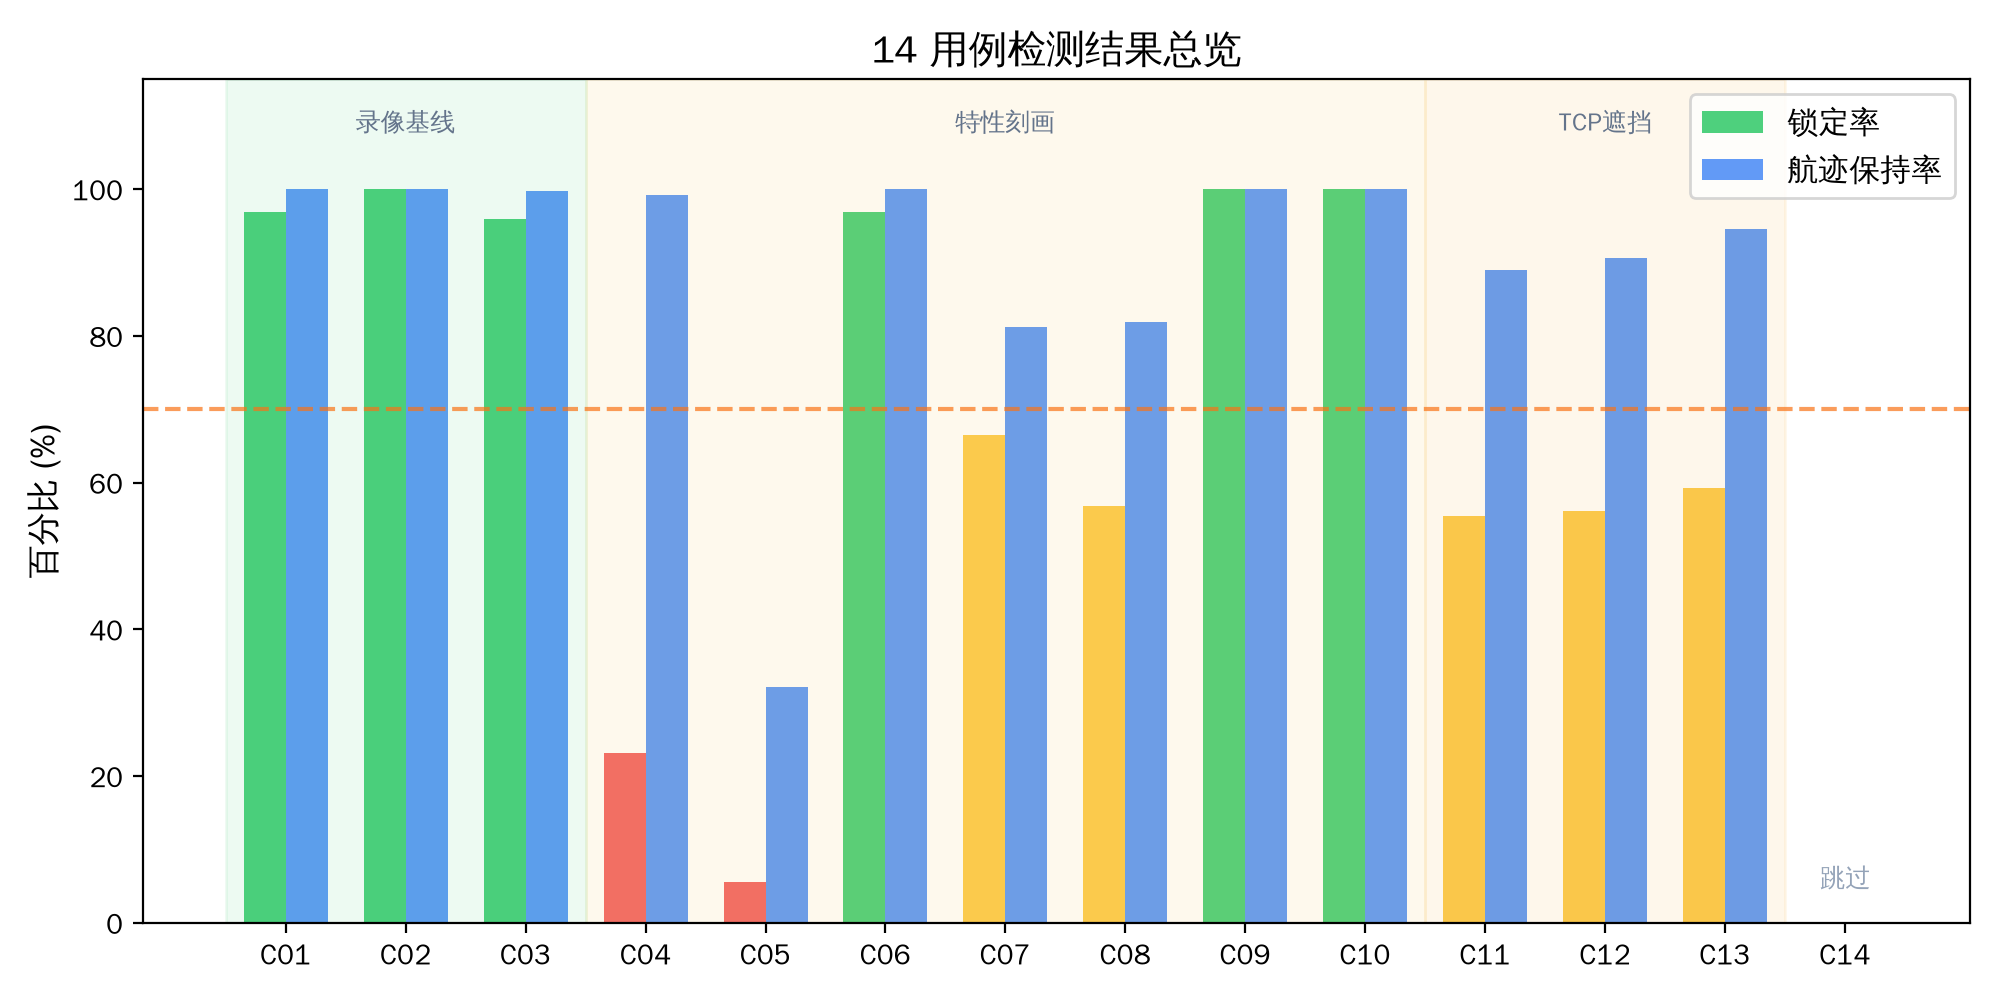
\includegraphics[width=0.9\textwidth]{G_chart_overview.png}
  \caption{14 用例锁定率与航迹保持率总览}
  \label{fig:overview}
\end{figure}

其中，锁定率定义为 LOCKED 帧占比（真实量测），
航迹保持率定义为 LOCKED + COAST 帧占比（含预测外推）。
两项指标的关系反映了状态机在目标遮挡场景下的补偿能力。

\subsection{仿真录像基线（C01--C03）}

C01--C03 使用仿真录像作为输入，验证系统的基本检测与跟踪能力。

\textbf{C01（仿真闭环基线）}：900 帧中 872 帧 LOCKED（96.9\%）、
28 帧 COAST，航迹保持率 100\%。置信度均值 0.550，
距离范围 3.0--6.2\,m，处理帧率 29.8\,fps。首帧即锁定（0.00\,s），
表明模型对仿真场景中的无人机目标具有即时检出能力。

\textbf{C02（早期标定版录像）}：900 帧全部 LOCKED（100\%），
置信度均值 0.855，距离范围 4.6--9.7\,m。该录像在早期标定阶段录制，
目标尺寸和光照条件较优，因此置信度较高。处理帧率 28.1\,fps。

\textbf{C03（长录像中后段）}：从同一录像的 30\,s 处开始播放，
900 帧中 864 帧 LOCKED（96.0\%）、34 帧 COAST、2 帧 SEARCHING，
保持率 99.8\%。首锁时间 0.07\,s。该用例验证了系统在长时间运行中的稳定性，
结果表明系统在 30\,s 偏移后仍能快速恢复锁定。

三例均通过合格标准（锁定率 $\geq 80\%$），
证明系统在仿真场景下具有稳定可靠的检测与跟踪能力。

\subsection{真实场景录像分析（C04--C05）}
\label{subsec:real_scenario}

C04 和 C05 使用外场真实场景录像，用于测试模型在真实环境中的泛化能力。
两例的锁定率均较低，但原因截然不同。

\subsubsection{C04：置信度波动导致的锁定振荡}

C04 的锁定率仅为 23.2\%，但航迹保持率高达 99.3\%。
深入分析发现：

\begin{itemize}
  \item 539 帧中 414 帧（76.8\%）检测器未输出检测框，
        有框帧的置信度均值仅 0.544（最低 0.205）；
  \item 状态转换 145 次，平均每 3.7 帧翻转一次，
        LOCKED 与 COAST 之间频繁振荡；
  \item 距离量测正常（4.4--8.9\,m），检测框尺寸合理
        （61--170\,px 宽），说明目标可见但模型置信度偏低。
\end{itemize}

根因分析：真实外场画面与仿真微调数据集之间存在域差异
（Domain Gap），导致模型在真实场景下的置信度普遍偏低
（0.2--0.3 附近波动），频繁触发 LOCKED$\leftrightarrow$COAST 状态转换。
然而，正是状态机的 COAST 机制（$T_{\text{coast}} = 1.0$\,s）
在频繁丢检时维持了 403/539 帧（74.8\%）的航迹显示，
将航迹保持率从 23.2\% 拉升至 99.3\%。

\textbf{此结果充分证明了状态机在低置信度场景下的核心价值}：
若采用原始的逐帧检测方案，76.8\% 的帧将显示无目标（数据断闪）；
而状态机靠 COAST 预测维持了连续的态势显示。

\subsubsection{C05：远距离小目标检出边界}

C05 的锁定率仅 5.6\%，航迹保持率 32.1\%。分析发现：

\begin{itemize}
  \item 539 帧中 509 帧（94.4\%）检测器未输出检测框；
  \item 距离 10.0--14.3\,m，检测框仅 50--80\,px 宽 $\times$ 22--30\,px 高
        （平均面积 1371\,px$^2$，约为 C04 的 1/4）；
  \item 有框帧的置信度均值 0.399（最高 0.703），多数帧在 0.2--0.3 徘徊；
  \item 372 帧 SEARCHING（69.0\%），目标完全丢失。
\end{itemize}

根因分析：目标距离超过 10\,m 时，检测框尺寸小于约 50\,px，
YOLOv8 的检出率急剧下降。按距离段细化分析：
10--12\,m 段 34 帧中仅 6 帧 LOCKED（17.6\%），
12--14\,m 段 125 帧中仅 24 帧 LOCKED（19.2\%），
但两段的航迹保持率均为 100\%（全部靠 COAST 预测维持）。
这是单目视觉检测的固有局限性：目标距离越远，成像尺寸越小，
可供模型辨识的特征越少。

C05 标定了本系统的适用距离上限（约 10\,m），
为实际部署中的相机选型和部署距离设计提供了参考依据。
需说明的是，仿真轨迹仅覆盖 3--10\,m，
10\,m 以上的性能数据完全依赖此真实场景录像，
仿真域内缺乏对应距离段的定量验证。

\subsection{置信度门限敏感性分析（C06--C08）}

C06--C08 使用同一仿真录像，仅改变置信度门限
（0.20 / 0.35 / 0.50），分析门限对检测性能的影响，
结果如图~\ref{fig:threshold} 所示。

\begin{figure}[H]
  \centering
  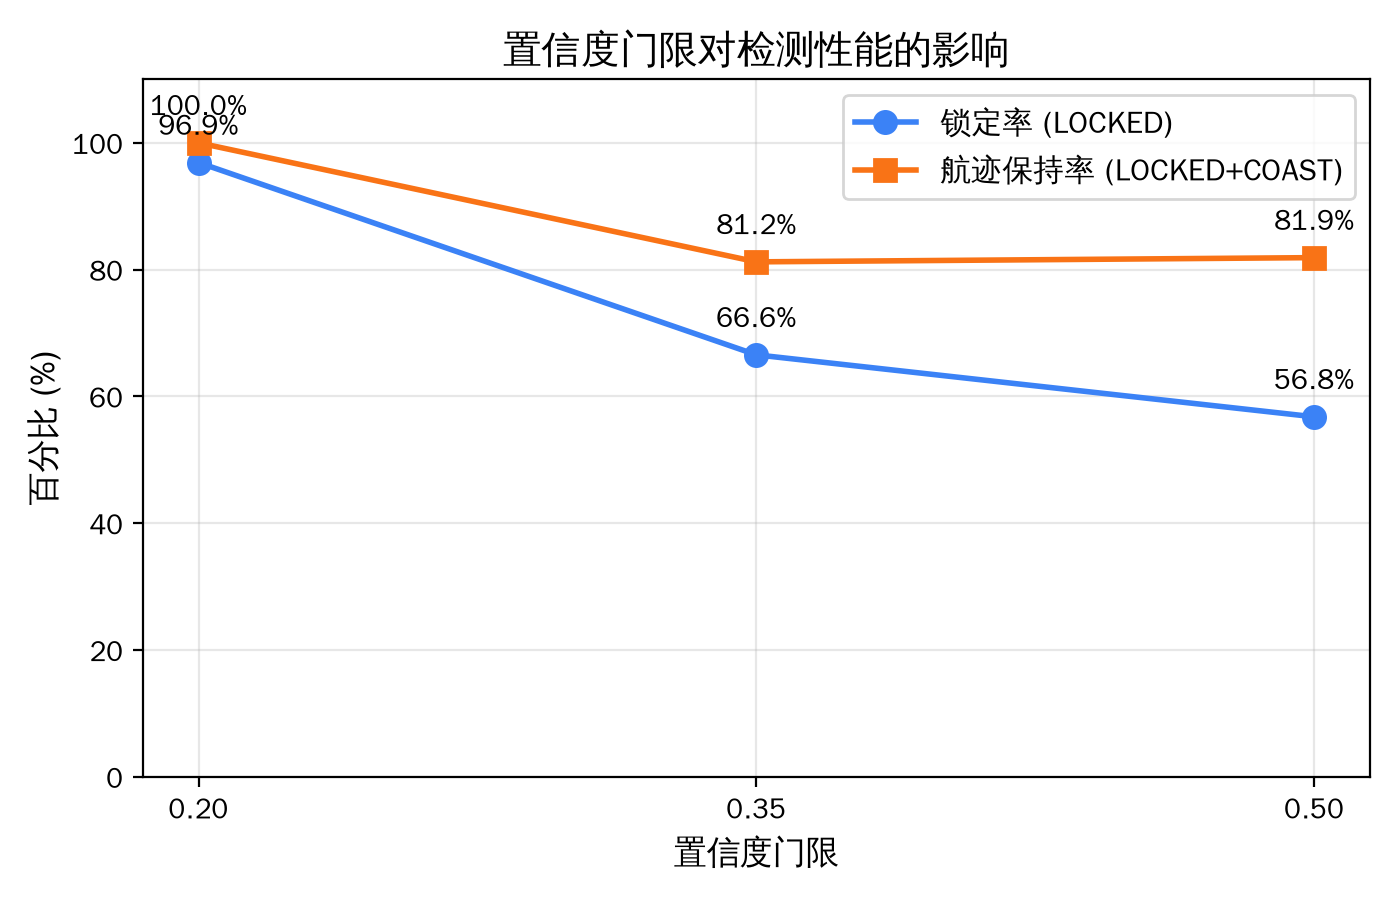
\includegraphics[width=0.75\textwidth]{G_chart_threshold_scan.png}
  \caption{置信度门限对锁定率与航迹保持率的影响}
  \label{fig:threshold}
\end{figure}

\begin{table}[H]
\centering
\caption{门限扫描结果}
\label{tab:threshold}
\begin{tabular}{ccccc}
\toprule
\textbf{门限} & \textbf{锁定率} & \textbf{保持率} & \textbf{置信度均值} & \textbf{处理fps} \\
\midrule
0.20 & 96.9\% & 100.0\% & 0.550 & 29.5 \\
0.35 & 66.6\% & 81.2\% & 0.661 & 35.8 \\
0.50 & 56.8\% & 81.9\% & 0.707 & 39.0 \\
\bottomrule
\end{tabular}
\end{table}

分析：

\begin{enumerate}
  \item \textbf{锁定率随门限升高而下降}：门限从 0.20 升至 0.50 时，
        锁定率从 96.9\% 降至 56.8\%。这是因为高门限过滤掉了
        大量低置信度的真实目标检测框，导致 LOCKED 状态频繁丢失。

  \item \textbf{航迹保持率的非线性变化}：保持率在门限 0.20 时为 100\%，
        在 0.35 和 0.50 时分别降至 81.2\% 和 81.9\%。
        注意 0.50 门限下的保持率（81.9\%）略高于 0.35（81.2\%），
        这是因为高门限下虽然 LOCKED 帧减少，但 COAST 机制补偿了
        部分丢失帧，且高门限过滤掉的假阳性检测框反而减少了
        状态机的误跳转。

  \item \textbf{处理帧率随门限升高而升高}：门限 0.20 时 29.5\,fps，
        门限 0.50 时 39.0\,fps。这是因为高门限下模型输出的检测框更少，
        后处理（NMS、状态机更新、卡尔曼滤波）的计算量更小。

  \item \textbf{门限 0.20 为最优选择}：在仿真场景中，门限 0.20
        实现了最高的锁定率（96.9\%）和保持率（100\%），
        且处理帧率（29.5\,fps）满足实时性要求。
\end{enumerate}

\subsection{等效尺寸敏感性分析（C09--C10）}

C09 和 C10 使用同一录像，仅改变无人机等效尺寸参数
（0.230\,m / 0.310\,m），分析其对测距结果的影响，
结果如图~\ref{fig:size} 所示。

\begin{figure}[H]
  \centering
  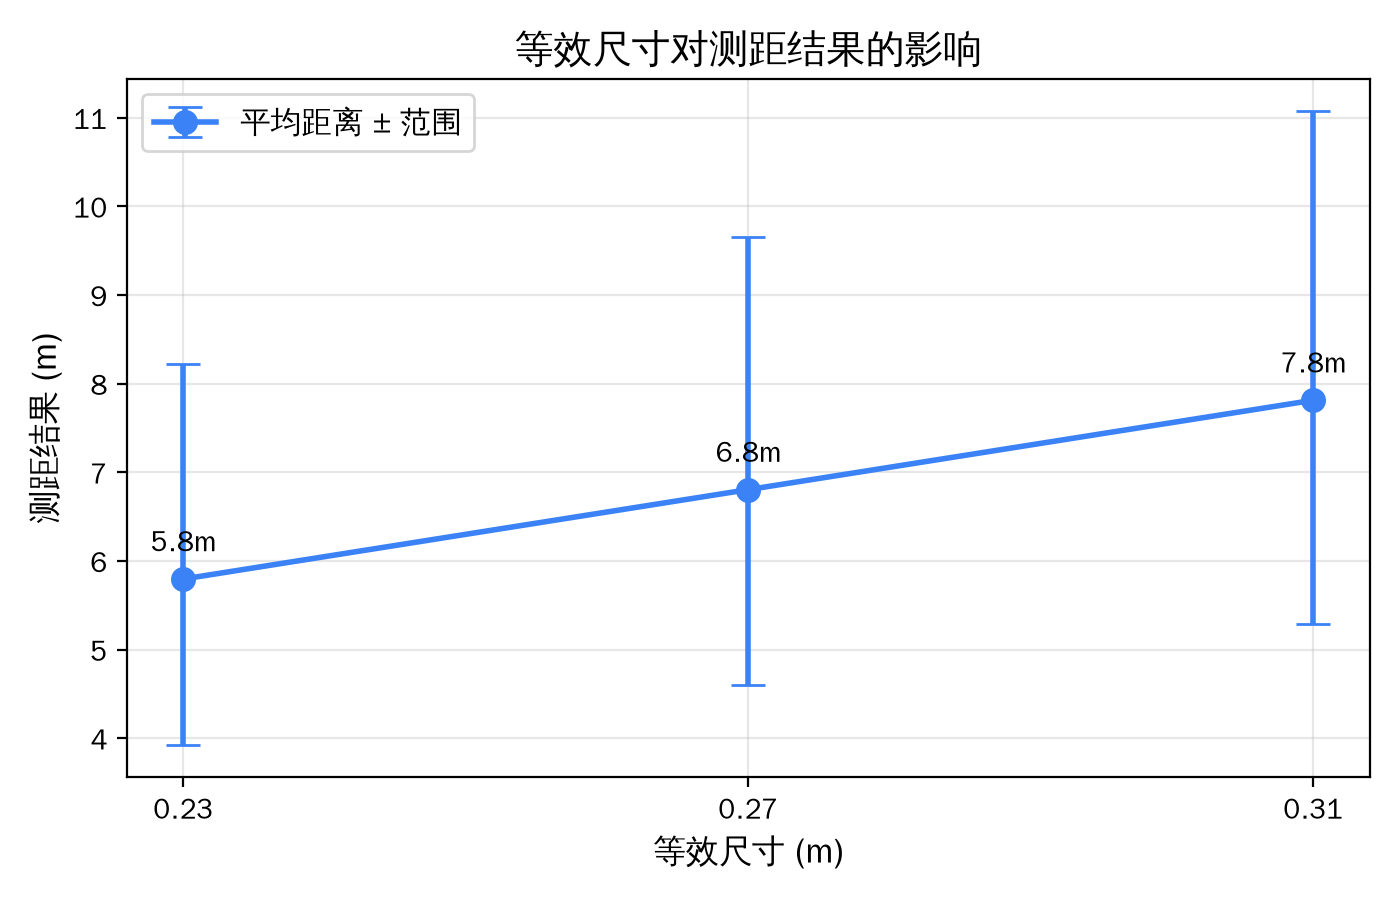
\includegraphics[width=0.75\textwidth]{G_chart_size_sensitivity.png}
  \caption{等效尺寸对测距结果的影响}
  \label{fig:size}
\end{figure}

\begin{table}[H]
\centering
\caption{尺寸敏感性结果}
\label{tab:size}
\begin{tabular}{ccccc}
\toprule
\textbf{尺寸(m)} & \textbf{距离范围(m)} & \textbf{平均距离(m)} & \textbf{锁定率} & \textbf{处理fps} \\
\midrule
0.230 & 3.9--8.2 & 5.8 & 100\% & 39.3 \\
0.270 & 4.6--9.7 & 6.8 & 100\% & 28.1 \\
0.310 & 5.3--11.1 & 7.8 & 100\% & 39.2 \\
\bottomrule
\end{tabular}
\end{table}

由式~(\ref{eq:range}) 可知，测距结果 $Z$ 与等效尺寸 $D_{\text{real}}$ 成正比。
实验结果验证了这一线性关系：

\begin{itemize}
  \item 尺寸从 0.230\,m 增至 0.310\,m（比例 $0.310/0.230 = 1.348$），
        平均距离从 5.8\,m 增至 7.8\,m（比例 $7.8/5.8 = 1.345$），
        几乎完全吻合理论比值。
  \item 距离范围随尺寸等比例扩大，最小值和最大值均按比例增长。
\end{itemize}

该结果证明了单目测距公式（式~\ref{eq:range}）的正确性，
同时也标定了等效尺寸参数对标定结果的影响：
尺寸偏差 10\%（如 0.270$\rightarrow$0.297\,m）将导致测距偏差约 10\%。
因此，精确测量目标无人机的等效尺寸对测距精度至关重要。

\subsection{TCP 实时遮挡场景分析（C11--C13）}
\label{subsec:tcp_occlusion}

C11--C13 在带有遮挡物的仿真场景下进行三轮 TCP 实时测试，
验证系统在目标频繁被遮挡条件下的跟踪鲁棒性。
三轮测试的状态分布如图~\ref{fig:tcp_state} 所示。

\begin{figure}[H]
  \centering
  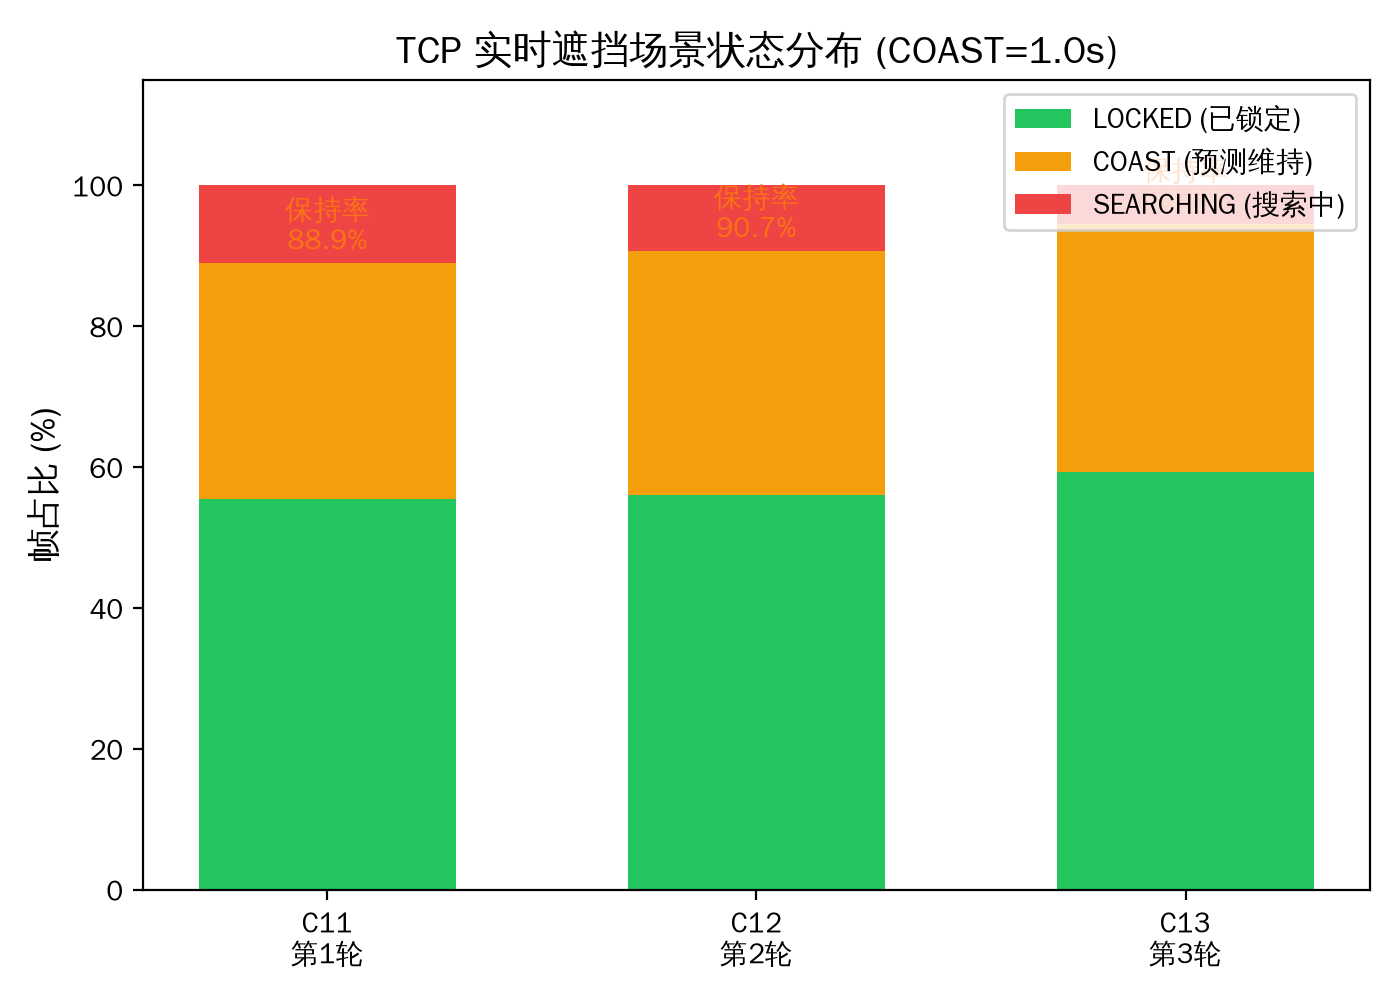
\includegraphics[width=0.75\textwidth]{G_chart_tcp_state_dist.png}
  \caption{TCP 遮挡场景三态分布（COAST=1.0\,s）}
  \label{fig:tcp_state}
\end{figure}

\begin{table}[H]
\centering
\caption{TCP 遮挡场景测试结果}
\label{tab:tcp}
\begin{tabular}{lccc}
\toprule
\textbf{指标} & \textbf{C11} & \textbf{C12} & \textbf{C13} \\
\midrule
总帧数 & 424 & 428 & 437 \\
LOCKED 帧 & 235 (55.4\%) & 240 (56.1\%) & 259 (59.3\%) \\
COAST 帧 & 142 (33.5\%) & 148 (34.6\%) & 154 (35.2\%) \\
SEARCHING 帧 & 47 (11.1\%) & 40 (9.3\%) & 24 (5.5\%) \\
航迹保持率 & 88.9\% & 90.7\% & 94.5\% \\
首锁时间 (s) & 0.00 & 0.00 & 0.21 \\
置信度均值 & 0.751 & 0.739 & 0.751 \\
距离范围 (m) & 2.8--7.1 & 2.0--7.2 & 2.2--6.1 \\
处理帧率 (fps) & 21.1 & 21.3 & 21.8 \\
结论 & PASS & PASS & PASS \\
\bottomrule
\end{tabular}
\end{table}

分析：

\begin{enumerate}
  \item \textbf{锁定率与遮挡事件}：三轮测试的锁定率在 55--59\% 之间，
        明显低于仿真录像基线（C01--C03 的 96--100\%）。
        这是因为目标无人机在随机航迹中频繁被建筑物、树木等遮挡物挡住，
        导致检测器无法输出检测框。COAST 帧占比高达 33--35\%，
        表明遮挡事件频繁发生。

  \item \textbf{航迹保持率}：尽管锁定率较低，但三轮测试的航迹保持率
        分别为 88.9\%、90.7\% 和 94.5\%，均远超 70\% 的合格标准。
        这说明 COAST 机制有效补偿了遮挡导致的检测中断，
        在目标不可见期间通过卡尔曼预测维持了航迹显示。

  \item \textbf{搜索态占比}：C11--C13 的 SEARCHING 帧占比分别为
        11.1\%、9.3\% 和 5.5\%，呈下降趋势。C13 的搜索帧最少（24 帧），
        首锁时间 0.21\,s，说明第三轮的航迹规划恰好使目标更多时间
        处于可见区域。这也从侧面验证了随机航迹的可复现性
        （种子化生成）和三轮测试间的差异性。

  \item \textbf{处理帧率}：TCP 实时链路的帧率约 21\,fps，
        低于录像回放的 28--39\,fps。这是因为 TCP 帧流需要经过
        网络传输和帧解码，引入了额外延迟。但 21\,fps 仍满足
        实时检测的基本要求。

  \item \textbf{距离范围}：三轮测试的距离范围分别为
        2.8--7.1\,m、2.0--7.2\,m 和 2.2--6.1\,m，
        动态范围较大，验证了随机航迹在近距离和远距离间的
        往复飞行能力。
\end{enumerate}

\subsection{COAST 预算优化分析}
\label{subsec:coast_opt}

在 TCP 遮挡场景测试中，发现 COAST 预算（$T_{\text{coast}}$）
对航迹保持率有显著影响。初始设置 $T_{\text{coast}} = 0.6$\,s 时，
多数遮挡事件的持续时间为 0.6--1.0\,s，刚好超过 COAST 预算，
导致频繁进入 SEARCHING 状态。重锁平均耗时 0.75--1.48\,s，
最长 3.03\,s。

将 $T_{\text{coast}}$ 从 0.6\,s 增至 1.0\,s 后，大部分遮挡事件
不再超时，航迹保持率显著提升，如图~\ref{fig:coast_opt} 所示。

\begin{figure}[H]
  \centering
  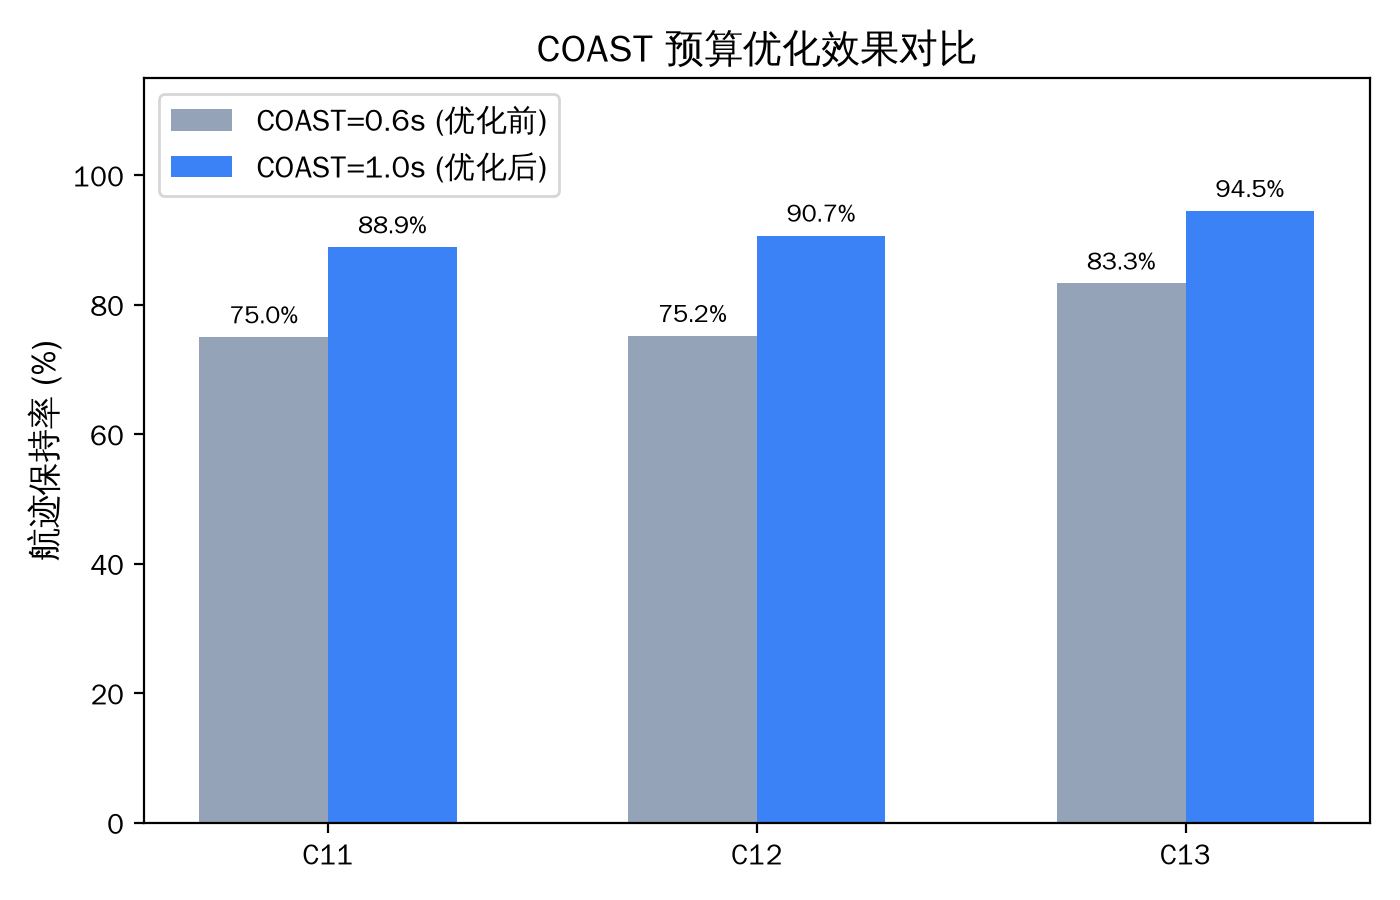
\includegraphics[width=0.7\textwidth]{G_chart_coast_optimization.png}
  \caption{COAST 预算优化效果对比}
  \label{fig:coast_opt}
\end{figure}

\begin{table}[H]
\centering
\caption{COAST 预算优化对比}
\label{tab:coast_opt}
\begin{tabular}{lccc}
\toprule
\textbf{指标} & \textbf{C11} & \textbf{C12} & \textbf{C13} \\
\midrule
保持率 ($T=0.6$\,s) & 75.0\% & 75.2\% & 83.3\% \\
保持率 ($T=1.0$\,s) & 88.9\% & 90.7\% & 94.5\% \\
提升幅度 & +13.9\% & +15.5\% & +11.2\% \\
\bottomrule
\end{tabular}
\end{table}

C12 的提升幅度最大（+15.5\%），因为其在 $T=0.6$\,s 时的
COAST 超时重锁平均耗时最长（1.48\,s），延长预算后
大部分遮挡不再超时。三轮测试的平均提升幅度为 +13.5\%。

这一结果说明，COAST 预算的设置应与场景中遮挡事件的
典型持续时间相匹配。过短会导致频繁进搜索态，
过长则可能在外推发散后仍保持错误航迹。
$T_{\text{coast}} = 1.0$\,s 在本文的仿真遮挡场景中取得了最优平衡。

\subsection{实时态势可视化}

图~\ref{fig:dashboard_sat} 展示了 TCP 实时检测中的目标态势页。
系统在检测到目标后，左栏目标卡片实时显示威胁等级（"高威胁"，
橙色标识）、置信度（0.81）和距离（4.4\,m）；
中间卫星图上标注目标位置点与蓝色航迹；
右侧罗盘指针指向目标方位（约 0°），中心大字号显示距离；
底部数据条 8 项指标全部实时刷新；
右下角 PIP（画中画）窗口显示带有绿色检测框的实时视频画面。

当距离 $< 5$\,m 时，系统自动将告警等级提升为"高威胁"
（橙色），罗盘告警环亮起；距离 $< 3$\,m 时升级为红色"紧急"。
这一分级告警机制为操作员提供了直观的态势感知。

雷达模式（图~\ref{fig:dashboard_radar}）将地图区域切换为
极坐标雷达显示，以 3\,m、5\,m、8\,m 为距离环，
蓝色三角标记本机位置，橙色圆点标记目标位置，
适用于无卫星图或强调相对距离的场景。

%% ====================================================================
\section{实验结论}
\label{sec:conclusion}
%% ====================================================================

\subsection{主要发现}

通过 14 个测试用例的系统化验证，本文得出以下主要结论：

\begin{enumerate}
  \item \textbf{仿真微调消除检测死区}：仿真域微调前，模型在 3--5\,m
        近距段和 9--10\,m 远距段的检出率均为 0\%（检测死区），
        有效工作窗口仅 7--9\,m。微调后，全距离段（3--10\,m）
        检出率提升至 100\%，死区完全消除。

  \item \textbf{仿真场景下的检测可靠性}：在固定轨迹、无遮挡的仿真录像中，
        系统达到了 96--100\% 的锁定率和 $\geq 99.8\%$ 的航迹保持率
        （C01--C03）；但在引入随机航迹与遮挡物的 TCP 实时场景中，
        锁定率降至 55--59\%，航迹保持率仍达 89--95\%（C11--C13），
        证明系统在复杂场景下具有可靠的跟踪能力。

  \item \textbf{状态机对遮挡的鲁棒性}：在带有遮挡物的 TCP 实时场景中，
        系统的锁定率为 55--59\%（目标可见时），
        但航迹保持率达到 89--95\%（含 COAST 预测），
        远超 70\% 的合格标准。COAST 机制在目标被遮挡期间
        通过卡尔曼预测维持了连续的航迹显示和距离数据输出。

  \item \textbf{状态机在低置信度场景的价值}：C04 的真实场景测试中，
        模型置信度普遍偏低（0.2--0.3），锁定率仅 23.2\%，
        但 COAST 机制将航迹保持率提升至 99.3\%。
        若采用逐帧检测方案，76.8\% 的帧将显示无目标，
        数据断闪严重。

  \item \textbf{COAST 预算优化}：将 $T_{\text{coast}}$ 从 0.6\,s
        增至 1.0\,s 后，航迹保持率平均提升 13.5\%，
        证明 COAST 预算应与场景遮挡事件的典型持续时间相匹配。

  \item \textbf{测距线性性验证}：等效尺寸敏感性测试（C09--C10）
        验证了单目测距公式 $Z = fD_{\text{real}}/D_{\text{pixel}}$
        的线性性，测距结果与尺寸参数成严格正比关系
        （实测比例 1.345 vs 理论比例 1.348，误差 $< 0.3\%$）。

  \item \textbf{系统适用边界}：C05 的测试结果标定了系统的
        适用距离上限（约 10\,m），当目标距离超过此值时，
        检测框尺寸 $< 50$\,px，YOLOv8 检出率急剧下降。
        这为实际部署中的相机选型和部署距离设计提供了参考。
\end{enumerate}

\subsection{局限性分析}

本系统存在以下局限性：

\begin{enumerate}
  \item \textbf{域差异}：模型在仿真场景下微调，对真实场景的
        泛化能力有限（C04 置信度 0.2--0.3）。可通过增加真实场景
        数据或采用域自适应算法改善。

  \item \textbf{距离限制与仿真覆盖范围}：单目测距在目标距离
        $> 10$\,m 时精度和检出率均显著下降（C05 真实场景：
        10--14\,m 段锁定率仅 17.6\%）。需说明的是，本文仿真轨迹
        仅覆盖 3--10\,m 距离范围，10\,m 以上的性能评估完全依赖
        真实场景录像 C05，仿真域内缺乏 10\,m+ 的定量验证数据。

  \item \textbf{处理帧率}：TCP 实时链路的帧率约 21\,fps，
        受网络传输和帧解码延迟影响，低于录像回放的 28--39\,fps。

  \item \textbf{单目标跟踪}：当前状态机仅支持单目标跟踪，
        多目标场景下需要扩展为多航迹管理（Multi-Object Tracking）。
\end{enumerate}

\subsection{未来工作}

基于本研究的实验结果和局限性，未来可从以下方向继续改进：

\begin{enumerate}
  \item \textbf{搜索态 ROI 缩小}：在 SEARCHING 状态下利用 COAST
        最后已知位置画搜索窗口，降低初锁门限，加速重锁。

  \item \textbf{多目标支持}：扩展状态机为多航迹管理，
        支持同时跟踪多架无人机。

  \item \textbf{域自适应}：在训练阶段引入真实场景数据或采用
        域随机化（Domain Randomization）技术，提升模型泛化能力。

  \item \textbf{硬件加速}：使用 TensorRT 等推理优化框架
        提升 GPU 推理帧率。

  \item \textbf{传感器融合}：引入雷达或激光雷达数据，
        通过多传感器融合突破单目视觉的距离限制。
\end{enumerate}

%% ====================================================================
%% 参考文献
%% ====================================================================

\begin{thebibliography}{99}

\bibitem{sod_yolov8}
B.~Khalili, A.~W.~Smyth.
SOD-YOLOv8: Enhancing YOLOv8 for Small Object Detection in Traffic Scenes.
\emph{arXiv preprint arXiv:2408.04786}, 2024.

\bibitem{msdf_net}
X.~Xiao, Y.~Lin, S.~Wang, et~al.
MSDF-Net: A Cross-Version Lightweight Detection Framework Based on Deformable Convolution and High-Resolution Feature Enhancement for Pine Wilt Disease.
\emph{Frontiers in Plant Science}, 2026.

\bibitem{ema}
O.~Ouyang, Y.~Liu, et~al.
Efficient Multi-Scale Attention Module with Cross-Spatial Learning.
In \emph{ICASSP}, 2023.

\bibitem{yolov8_mpeb}
W.~Xu, C.~Cui, Y.~Ji, et~al.
YOLOv8-MPEB Small Target Detection Algorithm Based on UAV Images.
\emph{PMC}, 2024.

\bibitem{yolov8}
J.~Redmon, A.~Farhadi.
YOLOv8: Ultralytics.
\url{https://github.com/ultralytics/ultralytics}, 2023.

\bibitem{faster_rcnn}
S.~Ren, K.~He, R.~Girshick, J.~Sun.
Faster R-CNN: Towards Real-Time Object Detection with Region Proposal Networks.
\emph{NeurIPS}, 2015.

\bibitem{ssd}
W.~Liu, et~al.
SSD: Single Shot MultiBox Detector.
\emph{ECCV}, 2016.

\bibitem{yolov5}
Ultralytics.
YOLOv5.
\url{https://github.com/ultralytics/yolov5}, 2020.

\bibitem{yolov12_adbc}
I.~Kurmashev, V.~Sememyuk, A.~Lupidi, et~al.
Study of the Optimal YOLO Visual Detector Model for Enhancing UAV Detection and Classification.
\emph{Drones}, 9(11):732, 2025.

\bibitem{rt_detr}
Y.~Zhao, et~al.
DETRs Beat YOLOs on Real-time Object Detection.
\emph{CVPR}, 2024.

\bibitem{radar_cuav}
L.~Xing, C.~Cui, M.~Wang, C.~Xu.
From Detection to Countermeasure: A Review of Key Technologies in Counter-UAV Systems.
\emph{IET Cyber-Systems and Robotics}, 8(1), 2026.

\bibitem{rf_drone}
D.~Aouladhadj, E.~Kpre, V.~Deniau, et~al.
Drone Detection and Tracking Using RF Identification Signals.
\emph{Sensors}, 23(17):7650, 2023.

\bibitem{rf_remoteid}
Y.~Tao, et~al.
Intelligent Multimodal Multi-Sensor Fusion-Based UAV Identification, Localization, and Countermeasures.
\emph{arXiv preprint arXiv:2510.22947}, 2025.

\bibitem{acoustic_drone}
Z.~Ghouli.
Passive Acoustic Detection and Localization of Drones Using MEMS Microphones and Machine Learning.
\emph{Acta Acustica}, 2026.

\bibitem{optical_cuav}
S.~Khazai, S.~Mirzaei.
A Comparative Analysis of YOLO and Faster R-CNN Algorithms for Micro-UAVs Detection in Surveillance Videos.
\emph{Earth Observation and Geomatics Engineering}, 2025.

\bibitem{fusion_cuav}
Y.~Dong, F.~Wu, S.~Zhang, et~al.
Securing the Skies: A Comprehensive Survey on Anti-UAV Methods, Benchmarking, and Future Directions.
\emph{arXiv preprint arXiv:2504.11967}, 2026.

\bibitem{px4}
PX4 Autopilot.
\url{https://px4.io/}, 2024.

\bibitem{jmavsim}
jMAVSim Simulator.
\url{https://github.com/PX4/PX4-Autopilot/tree/main/Tools/simulation/jmavsim}, 2024.

\bibitem{leaflet}
Leaflet: An Open-Source JavaScript Library for Mobile-Friendly Interactive Maps.
\url{https://leafletjs.com/}, 2024.

\bibitem{kalman}
R.~E.~Kalman.
A New Approach to Linear Filtering and Prediction Problems.
\emph{Journal of Basic Engineering}, 82(1):35--45, 1960.

\end{thebibliography}

%% ====================================================================
%% 附录 A：缩写词表
%% ====================================================================

\appendix
\section*{附录 A：缩写词表}
\label{sec:glossary}
\addcontentsline{toc}{section}{附录 A：缩写词表}

\begin{table}[H]
\centering
\caption{缩写词对照表}
\label{tab:glossary}
\small
\begin{tabular}{p{2.5cm}p{4cm}p{7cm}}
\toprule
\textbf{缩写} & \textbf{全称} & \textbf{含义说明} \\
\midrule
DRLS & Drone Recognition \& Localization System & 无人机识别与定位系统，本文设计的完整系统名称 \\
YOLO & You Only Look Once & 单阶段目标检测算法族 \\
YOLOv8n & YOLOv8 nano & YOLOv8 的轻量版本，参数量 3\,M 级 \\
P2 & P2 detection head (stride=4) & 高分辨率小目标检测层，下采样率为 4 \\
EMA & Efficient Multi-scale Attention & 高效多尺度注意力机制，用于特征通道重加权 \\
C2f & Convolution to Feature & YOLOv8 中的特征提取模块 \\
mAP & mean Average Precision & 平均精度均值，目标检测标准评价指标 \\
AP\_small & Average Precision (small) & 小目标平均精度，COCO 定义目标面积 $< 32 \times 32$\,px \\
FPS & Frames Per Second & 每秒处理帧数，衡量实时性 \\
IoU & Intersection over Union & 交并比，衡量检测框重叠程度 \\
NMS & Non-Maximum Suppression & 非极大值抑制，去重复检测框 \\
AKF & Adaptive Kalman Filter & 自适应卡尔曼滤波，本文用于距离平滑 \\
COAST & Coasting (prediction-only) & 预测维持状态，目标遮挡时卡尔曼外推 \\
SEARCH & Searching & 搜索状态，状态机初始态 \\
LOCKED & Locked & 锁定状态，稳定跟踪目标 \\
JUMP\_GATE & Jump Gate & 空间跳转门限，防止目标框跳到其他物体 \\
Z\_GATE & Z Gate & 距离跳变门限，拒绝异常距离量测 \\
CSV & Comma-Separated Values & 逗号分隔值文件格式，用于逐帧数据记录 \\
UDP & User Datagram Protocol & 用户数据报协议，用于实时数据输出 \\
TCP & Transmission Control Protocol & 传输控制协议，用于接收仿真帧流 \\
PX4 & PX4 Autopilot & 开源飞控系统 \\
jMAVSim & Java MAVLink Simulator & PX4 的 Java 仿真器 \\
SITL & Software In The Loop & 软件在环仿真 \\
MAVLink & Micro Air Vehicle Link & 无人机通信协议 \\
FOV & Field of View & 视场角 \\
RCS & Radar Cross Section & 雷达截面积 \\
RF & Radio Frequency & 射频 \\
TDOA & Time Difference of Arrival & 到达时间差，用于 RF 定位 \\
AOA & Angle of Arrival & 到达角度，用于 RF 定位 \\
LiDAR & Light Detection and Ranging & 激光雷达 \\
IR & Infrared & 红外 \\
PIR & Passive Infrared & 被动红外 \\
GPU & Graphics Processing Unit & 图形处理器，用于深度学习推理 \\
SOTA & State of the Art & 当前最优水平 \\
OOD & Out of Distribution & 分布外，指测试数据与训练数据分布不一致 \\
Det-Fly & Detection-Fly & 无人机检测数据集名称 \\
RCOL & Range-based Color table & 距离-颜色映射表，用于告警分级显示 \\
PIP & Picture in Picture & 画中画窗口 \\
QSS & Qt Style Sheet & Qt 样式表，用于界面美化 \\
JSON & JavaScript Object Notation & 轻量数据交换格式，用于配置持久化 \\
GUI & Graphical User Interface & 图形用户界面 \\
\bottomrule
\end{tabular}
\end{table}

\end{document}
